\documentclass[11pt, aspectratio=169]{beamer}

\usepackage{amsmath, amsfonts, microtype, nicefrac, amssymb, amsthm, centernot}

\usepackage{pgfpages}

\usepackage{helvet}
\usepackage[default]{lato}
\usepackage{array}

\usefonttheme[onlymath]{serif}

\usepackage[utf8]{inputenc}
\usepackage[T1]{fontenc}
\usepackage{textcomp}
\usepackage{bm}

\usepackage{mathpazo}
\usepackage{hyperref}
\usepackage{multimedia}
\usepackage{graphicx}
\usepackage{multirow}
\usepackage{graphicx}
\usepackage{dcolumn}
\usepackage{bbm}
\newcolumntype{d}[0]{D{.}{.}{5}}

\usepackage{graphicx}
\usepackage[space]{grffile}
\usepackage{booktabs}

\usepackage{setspace}

\usepackage{transparent}


%%% FIGURES %%%
\usepackage{caption, subcaption}
\usepackage{booktabs, siunitx}
\usepackage{pgfplots} 
%\usepackage[outdir=./figures]{epstopdf}
\usepackage{float}
\usepackage{graphicx}
\usepackage[absolute, overlay]{textpos}
\usepackage{epstopdf}


%%% TIKZ %%%
\usepackage{tikz}
\usepackage{verbatim}
\usetikzlibrary{arrows.meta}
\usetikzlibrary{positioning}
\usetikzlibrary{bending}
\usetikzlibrary{snakes}
\usetikzlibrary{calc}
\usetikzlibrary{arrows}
\usetikzlibrary{decorations.markings}
\usetikzlibrary{shapes.misc}
\usetikzlibrary{matrix, shapes, arrows, fit, tikzmark}


%%% ALGORITHM %%%
\usepackage{algorithm}
\usepackage[noend]{algpseudocode}
\usepackage{multimedia}


%%% APPENDIX SLIDE NUMBERING %%%
\usepackage{appendixnumberbeamer}


%%% BEAMER BUTTON %%%
%\setbeamertemplate{button}{\tikz
	%\node[
	%	inner xsep = 2pt, 
	%	draw = structure!0, 
	%	fill = myblue, 
	%	rounded corners = 4pt]{\color{white} \tiny\insertbuttontext};
	%}


%%% COLORS %%%
\definecolor{blue}{RGB}{0,38,118}
\definecolor{red}{RGB}{213,94,0}
\definecolor{yellow}{RGB}{240,228,66}
\definecolor{green}{RGB}{0,158,115}

\definecolor{myred}{RGB}{163,32,45}
\definecolor{navyblue}{rgb}{0.05,0.2,0.70}
\definecolor{myblue}{RGB}{0,51,150}
\definecolor{myorange}{RGB}{255,140,0}
\definecolor{myref}{RGB}{160,160,160}
\definecolor{shock}{RGB}{0, 125, 34}%{50, 168, 82}

\definecolor{background}{RGB}{255,253,218}

% Define a new transparent color
\definecolor{trans}{rgb}{1,1,1}
\colorlet{trans}{black!20} % 0 percent opacity

\hypersetup{
  colorlinks=false,
  linkbordercolor = {white},
  linkcolor = {blue}
}

\setbeamercolor{frametitle}{fg=blue}
\setbeamercolor{title}{fg=black}
\setbeamertemplate{footline}[frame number]
\setbeamertemplate{navigation symbols}{} 
\setbeamertemplate{itemize items}{-}
\setbeamercolor{itemize item}{fg=blue}
\setbeamercolor{itemize subitem}{fg=blue}
\setbeamercolor{enumerate item}{fg=blue}
\setbeamercolor{enumerate subitem}{fg=blue}
\setbeamercolor{button}{bg=background, fg=blue,}

%\setbeamercolor{background canvas}{bg=background}


%%% FRAME TITLE %%%
\setbeamerfont{title}{series=\bfseries, parent=structure}
\setbeamerfont{frametitle}{series=\bfseries, parent=structure}


%%% TRANSITION FRAME %%%
\newenvironment{transitionframe}{
	\setbeamercolor{background canvas}{bg=blue}
	\begin{frame}
		\thispagestyle{empty}
		\addtocounter{framenumber}{-1}
		\vspace{42mm}
		\hspace{4mm} }{
		\begin{tikzpicture}
			\tikz \fill [white] (1,6) rectangle (20,10);
		\end{tikzpicture}
	\end{frame}
}


%%% OUTLINE %%%
\AtBeginSection[]
{
	\begin{frame}
       \frametitle{Roadmap of Talk}
       \tableofcontents[currentsection]
   \end{frame}
}
\setbeamercolor{section in toc}{fg=blue}
\setbeamercolor{subsection in toc}{fg=red}
\setbeamersize{text margin left=1em,text margin right=1em} 


%%% ENVIRONMENTS
\newenvironment{witemize}{\itemize\addtolength{\itemsep}{10pt}}{\enditemize}

\makeatother
\setbeamertemplate{itemize items}{\large\raisebox{0mm}{\textbullet}}
\setbeamertemplate{itemize subitem}{\footnotesize\raisebox{0.15ex}{--}}
\setbeamertemplate{itemize subsubitem}{\Tiny\raisebox{0.7ex}{$\blacktriangleright$}}

\setbeamertemplate{enumerate item}[default]
\setbeamertemplate{enumerate subitem}{\textbullet}
\makeatletter

% ITEMIZE SPACING:
% \usepackage{xpatch}
% \xpatchcmd{\itemize}
% {\def\makelabel}
% {\setlength{\itemsep}{0mm}\def\makelabel}
% {}
% {}


%%% PRETTY ENUMERATE %%%
% \usepackage{stackengine,xcolor}
% \newcommand\circnum[2]{\stackinset{c}{}{c}{.1ex}{\small\textcolor{white}{#2}}%
	% 	{\abovebaseline[-.7ex]{\Huge\textcolor{#1}{$\bullet$}}}}
% \newenvironment{myenum}
% {\let\svitem\item
	% 	\renewcommand\item[1][black]{%
		% 		\refstepcounter{enumi}\svitem[\circnum{##1}{\theenumi}]}%
	% 	\begin{enumerate}}{\end{enumerate}}
\usepackage{stackengine,xcolor,graphicx}
\newcommand\circnum[2]{\smash{\stackinset{c}{}{c}{.2ex}{\small\textcolor{white}{#2}}%
		{\abovebaseline[-1.1ex]{\Huge\textcolor{#1}{\scalebox{1.5}{$\bullet$}}}}}}
\newenvironment{myenum}
{\let\svitem\item
	\renewcommand\item[1][black]{%
		\refstepcounter{enumi}\svitem[\circnum{##1}{\theenumi}]}%
	\begin{enumerate}}{\end{enumerate}}

\newcommand{\notimplies}{\;\not\!\!\!\implies}


%%% BEN'S SHORTCUTS %%%
\newcommand{\bi}{\begin{itemize}}
\newcommand{\ei}{\end{itemize}}
\newcommand{\be}{\begin{enumerate}}
\newcommand{\ee}{\end{enumerate}}
\newcommand{\bd}{\begin{description}}
\newcommand{\ed}{\end{description}}
\definecolor{gred}{RGB}{200,0,25}
\definecolor{gblue}{RGB}{25,0,200}
\definecolor{ggreen}{RGB}{25,200,25}
\definecolor{dgreen}{rgb}{0,0.5,0}
\definecolor{gpink}{RGB}{255,0,247}

\definecolor{foreground}{RGB}{0,0,0}
\definecolor{background}{RGB}{255,255,255}
%\definecolor{title}{RGB}{37,47,141}
\definecolor{title}{RGB}{0,0,0}
%\definecolor{title}{RGB}{25,0,200}
\definecolor{gray}{RGB}{155,155,155}
%\definecolor{subtitle}{RGB}{128,128,128}
\definecolor{subtitle}{RGB}{0,0,0}
\definecolor{hilight}{RGB}{102,255,204}
\definecolor{vhilight}{RGB}{255,111,207}

\newtheorem{assumption}{Assumption}
\newtheorem{condition}{Condition}
\newcommand{\tw}{\textcolor{white} }
\newcommand{\tblk}{\textcolor{black} }
\newcommand{\tr}{\textcolor{gred} }
\newcommand{\tb}{\textcolor{gblue} }
\newcommand{\tg}{\textcolor{dgreen} }
\newcommand{\tp}{\textcolor{gpink} }

\usepackage{ushort}



%%%%%%%%%%%%%%%%%%%%%%%%%%  TITLE   %%%%%%%%%%%%%%%%%%%%%%%%%%%%%%%%
\title[]{\\[8pt]
	{\large \color{blue} Dynamic Programming and Applications \\[5pt] \normalfont{Heterogeneous Agents and Inequality} \\[10pt] \normalfont{Lecture 11}}}
\author[Schaab]{Andreas Schaab}
\institute{}
\subject{}
\date{}



%%%%%%%%%%%%%%%%%%%%%%%%  BEGIN DOC   %%%%%%%%%%%%%%%%%%%%%%%%%%%%%%%
\begin{document}

%%% TIKZ %%% 
\tikzstyle{every picture}+=[remember picture]
%\everymath{\displaystyle}

\tikzset{   
	every picture/.style={remember picture,baseline},
	every node/.style={anchor=base,align=center,outer sep=1.5pt},
	every path/.style={thick},
}
\newcommand\marktopleft[1]{%
	\tikz[overlay,remember picture] 
	\node (marker-#1-a) at (-.3em,.3em) {};%
}
\newcommand\markbottomright[2]{%
	\tikz[overlay,remember picture] 
	\node (marker-#1-b) at (0em,0em) {};%
}
\tikzstyle{every picture}+=[remember picture] 
\tikzstyle{mybox} =[draw=black, very thick, rectangle, inner sep=10pt, inner ysep=20pt]
\tikzstyle{fancytitle} =[draw=black,fill=red, text=white]


\addtocounter{framenumber}{-1}
\thispagestyle{empty}
\maketitle 
\newpage



%%%%%%%%%%%%%%%%%%%%%%%%%%  SLIDE   %%%%%%%%%%%%%%%%%%%%%%%%%%%%%%%%
\begin{frame}{Outline}
\thispagestyle{empty}
\addtocounter{framenumber}{-1}

Part 2: Huggett (1993) in continuous time (Bewley-Huggett-Aiyagari)

\vspace{2mm}
\textit{This is the textbook heterogeneous agent model / standard incomplete markets model}

\vspace{2mm}
\begin{enumerate}
\item Households, firms and market clearing

\item Competitive equilibrium in sequence form

\item Recursive representation using dynamic programing

\item Competitive equilibrium in recursive form

\item Stationary competitive equilibrium in recursive form
\end{enumerate}


\vspace{8mm}
I learned all this from Benjamin Moll!

{\footnotesize \textit{Income and Wealth Distribution in Macroeconomics: A Continuous-Time Approach}}
 
\vspace{3mm}
See also Ben's teaching material: \url{https://benjaminmoll.com/lectures/}

% Part 3: Theoretical properties of the HA model (continuous > discrete time)
% 
% \vspace{3mm}
% Paper: \textit{Income and Wealth Distribution in Macroeconomics: A Continuous-Time Approach}
% 
% \vspace{1mm}
% Slides based on Ben's: \url{https://benjaminmoll.com/lectures/}
\end{frame}


%%%%%%%%%%%%%%%%%%%%%%%%%%  SLIDE   %%%%%%%%%%%%%%%%%%%%%%%%%%%%%%%%
\begin{transitionframe}
	{\color{white} \Huge \textbf{Part 2: Huggett (1993)} \vspace{2mm}}
\end{transitionframe}



%%%%%%%%%%%%%%%%%%%%%%%%%%  SLIDE   %%%%%%%%%%%%%%%%%%%%%%%%%%%%%%%%
\begin{frame}{Model overview}
\begin{witemize}
\item Time is continuous, $t \in [0, \infty)$

\item No aggregate uncertainty $\implies$ focus on one-time, unanticipated (``MIT'') shocks (perfect foresight wrt. macroeconomic aggregates)

\item Two types of agents: continuum of households (measure 1) + representative firm

\item Households face ``uninsurable idiosyncratic income risk''

\item There is a single riskfree asset in zero net supply ($\sim$ government bond)

\end{witemize}

\vspace{4mm} 
\textbf{Plan:}
\begin{enumerate}
\item Present model in sequence form focusing exposition on individual $i$
\item Recursive representation of competitive equilibrium
\end{enumerate}
\end{frame}


%%%%%%%%%%%%%%%%%%%%%%%%%%  SLIDE   %%%%%%%%%%%%%%%%%%%%%%%%%%%%%%%%
\begin{frame}{Households}

\vspace{3mm}
\textbf{Preferences.} The individual lifetime utility of a household $i \in [0, 1]$ is 
\begin{equation*}
	V_{i, 0} = \max_{ \{c_{i, t}\}_{t \geq 0} } \; \mathbb E_0 \int_0^\infty e^{- \rho t} u(c_{i, t}) dt
\end{equation*}


\vspace{5mm}
\textbf{Budget} and \textbf{borrowing constraints}:
\begin{align*}
	\dot a_{i, t} &= w_t y_{i, t} + r_t a_{i, t} - c_{i, t} \\[2pt]
	a_{i, t} &\geq \underline a
\end{align*}


\vspace{5mm}
\textbf{Idiosyncratic income risk}: each $y_{i, t}$ follows a Markov chain (later: diffusion)
\begin{equation*}
	y_{i, t} \in \{y_1, y_2\} \; \text{ Poisson with intensities } \lambda_1, \lambda_2
\end{equation*}

\end{frame}


%%%%%%%%%%%%%%%%%%%%%%%%%%  SLIDE   %%%%%%%%%%%%%%%%%%%%%%%%%%%%%%%%
\begin{frame}{}

\vspace{5mm}
\textbf{Definition.} The problem of household $i$ (in sequence form) is 
\begin{equation*}\label{HH}\begin{split}
	\max_{\{c_{i, t}\}_{t \geq 0}} \, 
		& \mathbb E_0 \int_0^\infty e^{-\rho t} u(c_{i, t}) dt \quad \quad \mbox{s.t.} \\[2pt]
		&\dot a_{i, t} = w_t y_{i, t} + r_t a_{i, t} - c_{i, t} \\[4pt]
		&y_{i, t} \in \{y_1, y_2\} \ \mbox{Poisson with intensities} \ \lambda_1,\lambda_2\\[4pt]
		&a_{i, t} \geq \ushort a \end{split}
\end{equation*}

\vspace{2mm}
\noindent
taking as given initial $(a_{i, 0}, y_{i, 0})$

\vspace{4mm}
\noindent
A \textbf{solution} to the household problem is a stochastic process $\{c_{i, t}, a_{i, t}\}_{t \geq 0}$
\end{frame}


%%%%%%%%%%%%%%%%%%%%%%%%%%  SLIDE   %%%%%%%%%%%%%%%%%%%%%%%%%%%%%%%%
\begin{frame}{Firms}

\begin{witemize}
\item A representative firm produces the (homogeneous) final consumption good using technology 
\begin{equation*}
	Y_t = A_t \ell_t
\end{equation*}

\item Firms are small and perfectly competitive $\implies$ firm problem is
\begin{equation*}
	\max_{\ell_t} Y_t - w_t \ell_t
\end{equation*}

\item Firm problem is \textbf{static} $\implies$ otherwise we would have to think hard about ownership
\end{witemize}

\end{frame}


%%%%%%%%%%%%%%%%%%%%%%%%%%  SLIDE   %%%%%%%%%%%%%%%%%%%%%%%%%%%%%%%%
\begin{frame}{Markets}

How many markets are there?

\pause
\vspace{4mm}
\noindent
\textbf{Goods market}:
\begin{equation*}
	Y_t = \int_0^1 c_{i, t} di
\end{equation*}


\vspace{4mm}
\noindent
\textbf{Labor market}:
\begin{equation*}
	\ell_t = \int_0^1 y_{i, t} di
\end{equation*}

\vspace{4mm}
\noindent
\textbf{Asset market}:
\begin{equation*}
	0 = \int_0^1 a_{i, t} di
\end{equation*}

\end{frame}


%%%%%%%%%%%%%%%%%%%%%%%%%%  SLIDE   %%%%%%%%%%%%%%%%%%%%%%%%%%%%%%%%
\begin{frame}{Competitive Equilibrium}

\vspace{6mm}
\noindent
\textbf{Definition.} (Competitive equilibrium: sequence form) 
\textit{
	Taking as given an initial distribution of assets and individual labor productivities $\{a_{i, 0}, y_{i, 0}\}_i$ as well as an exogenous path for TFP $\{A_t\}$, a competitive equilibrium comprises an allocation $\{Y_t, \ell_t, c_{i, t}, a_{i, t}\}$ and prices $\{r_t, w_t\}$ such that: (i) households optimize, (ii) firms optimize, and (iii) markets clear.
}

\pause
\vspace{8mm}
\begin{witemize}
\item Always show definition of your equilibrium!

\item Why is this a definition of competitive equilibrium ``in sequence form''?

\item How many parts are there to this definition?
\end{witemize}

\end{frame}


%%%%%%%%%%%%%%%%%%%%%%%%%%  SLIDE   %%%%%%%%%%%%%%%%%%%%%%%%%%%%%%%%
\begin{frame}{Recursive representation}
\begin{witemize}
\item This is the full model. Would you know how to solve it?

\pause
\item One theme of this course: recursive > sequence

\item Let's think hard: what does it take to bring this GE model into recursive form?

\pause
\item Right now: model = stochastic processes for each $i$

Recursive representation = functions over state variables

\item What about the household problem in PE? What are the state variables? Firms?

\vspace{1mm}
{\small \textit{What's the difference between PE and GE?}}

\pause
\item What about markets and GE? What does $\int_0^1 c_{i, t} di$ mean?

\end{witemize}
\end{frame}


%%%%%%%%%%%%%%%%%%%%%%%%%%  SLIDE   %%%%%%%%%%%%%%%%%%%%%%%%%%%%%%%%
\begin{frame}{}

\vspace{5mm}
Recall household problem: Given $(a_{i, 0}, y_{i, 0})$,
\begin{equation*}\label{HH}\begin{split}
	\max_{\{c_{i, t}\}_{t \geq 0}} \, 
		& \mathbb E_0 \int_0^\infty e^{-\rho t} u(c_{i, t}) dt \quad \quad \mbox{s.t.} \\[2pt]
		&\dot a_{i, t} = w_t y_{i, t} + r_t a_{i, t} - c_{i, t} \\[4pt]
		&y_{i, t} \in \{y_1, y_2\} \ \mbox{Poisson with intensities} \ \lambda_1,\lambda_2\\[4pt]
		&a_{i, t} \geq \ushort a \end{split}
\end{equation*}


\pause
\vspace{6mm}
\noindent
\textbf{Recursive representation}:
\begin{equation*}
	\rho V_t(a, y) = \max_c \bigg\{ u(c) + \mathbb E_t \frac{d V_t(a, y)}{dt} \bigg\}
\end{equation*}

\vspace{2mm}
Two \textbf{Q}s: What is $\mathbb E_t \frac{d V_t(a, y)}{dt}$? And what about borrowing constraint? 
\end{frame}


%%%%%%%%%%%%%%%%%%%%%%%%%%  SLIDE   %%%%%%%%%%%%%%%%%%%%%%%%%%%%%%%%
\begin{frame}{}

From previous slide:
\begin{equation*}
	\rho V_t(a, y) = \max_c \bigg\{ u(c) + \mathbb E_t \frac{d V_t(a, y)}{dt} \bigg\}
\end{equation*}


\vspace{6mm}
\textbf{Q1}: What is continuation value?
\pause
\begin{equation*}
	\rho V_t(a, y_j) = \max_c \bigg\{ u(c) + (r_t a + w_t y_j - c) \partial_a V_t(a, y_j) + \lambda_j(V_t(a, y_{-j}) - V_t(a, y_j)) + \partial_t V_t(a, y_j) \bigg\}
\end{equation*}


\vspace{4mm}
Resolving max operator gives FOC, which defines \textbf{consumption policy function}:
\begin{equation*}
	u'(c_t(a, y_j)) = \partial_a V_t(a, y_j)
\end{equation*}
for all $a$ and $j$. Define \textbf{savings policy function} as $s_t(a, y_j) = r_t a + w_t y_j - c_t(a, y_j)$

\end{frame}


%%%%%%%%%%%%%%%%%%%%%%%%%%  SLIDE   %%%%%%%%%%%%%%%%%%%%%%%%%%%%%%%%
\begin{frame}{}

\vspace{6mm}
\textbf{Q2}: Where is the borrowing constraint $a_{i, t} \geq \underline a$ in the HJB?

\vspace{2mm}
\textbf{Answer}: in the boundary condition!


\vspace{4mm}
\begin{witemize}
\item Borrowing constraint gives rise to \textbf{state constraint boundary condition} 
\begin{equation*}
	\partial_a V_t(\underline a, y_j) \geq u'(r_t \underline a + w_t y_j) 
\end{equation*}

\item Economic intuition: value of saving must be weakly larger than value of consuming

\item Heuristic derivation: the FOC still holds at the borrowing constraint
\begin{equation*}
	u'(c_t(\underline a, j)) = \partial_a V_t(a, y_j) 
\end{equation*}

\item But borrowing constraint requires that 
\begin{equation*}
	s_t(\underline a, y_j) = r_t \underline a + w_t y_j - c_t(\underline a, y_j) \geq 0
\end{equation*}

\item Borrowing constraint showing up as boundary condition = major advantage of continuous time!

\end{witemize}

\end{frame}



%%%%%%%%%%%%%%%%%%%%%%%%%%  SLIDE   %%%%%%%%%%%%%%%%%%%%%%%%%%%%%%%%
\begin{frame}{}

\textbf{Summary}: A solution to the household problem in \textbf{recursive form} is a set of two functions $V_t(a, y)$ and $c_t(a, y)$ that satisfy
\begin{equation*}
	\rho V_t(a, y_j) = u(c_t(a, y_j)) + (r_t a + w_t y_j - c_t(a, y_j)) \partial_a V_t(a, y_j) + \lambda_j(V_t(a, y_{-j}) - V_t(a, y_j)) + \partial_t V_t(a, y_j)
\end{equation*}
\begin{equation*}
	u'(c_t(a, y_j)) = \partial_a V_t(a, y_j)
\end{equation*}
with HJB boundary condition 
\begin{equation*}
	\partial_a V_t(\underline a, y_j) \geq u'(r_t \underline a + w_t y_j) 
\end{equation*}
To save space, will now use savings policy function $s_t(a, y_j) \equiv r_t a + w_t y_j - c_t(a, y_j)$ as shorthand

\end{frame}


%%%%%%%%%%%%%%%%%%%%%%%%%%  SLIDE   %%%%%%%%%%%%%%%%%%%%%%%%%%%%%%%%
\begin{frame}{Income and Wealth Distribution}

\begin{witemize}
\item We now have recursive representations of the household (and firm) problem 

\item But how do we do GE? We have conditions like $Y_t = \int_0^1 c_{i, t} di$

\item Instead, we want to get \textbf{aggregate consumption} by integrating over $c_t(a, y)$

\item Issue: there may be many households $i$ in state $(a, y)$! Remember (important): household $i$ is \textbf{uniquely} identified by her states $(a_i, y_i)$ in this model

\item Solution: integrate against the joint density $\sim$ income-wealth distribution $g_t(a, y)$:
\begin{equation*}
	Y_t = \iint c_t(a, y) g_t(a, y) \, da \, dy \equiv \sum_j \int c_t(a, y_j) g_t(a, y_j) da
\end{equation*}
\end{witemize}
\end{frame}



%%%%%%%%%%%%%%%%%%%%%%%%%%  SLIDE   %%%%%%%%%%%%%%%%%%%%%%%%%%%%%%%%
\begin{frame}{Kolmogorov Forward Equation}

\begin{witemize}
\item If we knew $g_t(a, y)$, we'd be done! Why?

\pause	
\item Notice: $g_t(a, y)$ is a new object that wasn't part of the eq. definition in sequence form 

$\implies$ Need new equilibrium condition!

\item Where does this equilibrium condition come from?

\pause
$\implies$ $g_t(a, y)$ must be consistent with household behavior

\item Turns out: $g_t(a, y)$ solves a \textbf{Kolmogorov forward equation}

\item Another major advantage of continuous time!

\end{witemize}
\end{frame}


%%%%%%%%%%%%%%%%%%%%%%%%%%  SLIDE   %%%%%%%%%%%%%%%%%%%%%%%%%%%%%%%%
\begin{frame}{}

\vspace{4mm}
{\color{blue} \textbf{Result}}: the joint density $g_t(a, y)$ solves the Kolmogorov forward (KF) equation
\begin{equation*}
	\partial_t g_t(a, y_j) = -\partial_a \Big[ (r_t a + w_t y_j - c_t(a, y_j)) g_t(a, y_j) \Big] - \lambda_j g_t(a, y_j) + \lambda_{-j} g_t(a, y_{-j}) 
\end{equation*}


\vspace{6mm}
\textbf{Proof}:
Define aggregate consumption as cross-sectional average consumption
\begin{equation*}
	C_t = \mathbb E_i (c_{i, t}) = \mathbb E_g(c_t(a, y)) \equiv \iint c_t(a, y) g_t(a, y) \, da \, dy
\end{equation*}
By ``Ito's lemma'', we have 
\begin{equation*}
	d c_t(a, y_j) = \partial_t c_t(a, y_j) dt + s_t(a, y_j) \partial_a c_t(a, y_j) dt + \lambda_j (c_t(a, y_{-j}) - c_t(a, y_j)) dt 
\end{equation*}
\end{frame}


%%%%%%%%%%%%%%%%%%%%%%%%%%  SLIDE   %%%%%%%%%%%%%%%%%%%%%%%%%%%%%%%%
\begin{frame}{}
On the \textbf{one hand}, we have
\begin{equation*}
	d C_t = \mathbb E_g(dc_t(a, y)) = \iint d c_t(a, y) g_t(a, y) \, da \, dy
\end{equation*}
and so plugging in 
\begin{equation*}
	= \sum_j \int \bigg[ \partial_t c_t(a, y_j) + s_t(a, y_j) \partial_a c_t(a, y_j) + \lambda_j (c_t(a, y_{-j}) - c_t(a, y_j)) \bigg] g_t(a, y_j) \, da \, dt
\end{equation*}


\vspace{4mm}
On the \textbf{other hand}, we have
\begin{equation*}
	d C_t = d \iint c_t(a, y) g_t(a, y) \, da \, dy = \sum_j \int \bigg[ g_t(a, y_j) \partial_t c_t (a, y_j) + c_t(a, y_j) \partial_t g_t(a, y_j) \bigg] \, da dt
\end{equation*}


\vspace{4mm}
We now \textbf{equate the two} (next slide)
\end{frame} 


%%%%%%%%%%%%%%%%%%%%%%%%%%  SLIDE   %%%%%%%%%%%%%%%%%%%%%%%%%%%%%%%%
\begin{frame}{}
\begin{equation*}
	0 = \sum_j \int \bigg\{
	\bigg[ s_t(a, y_j) \partial_a c_t(a, y_j) + \lambda_j (c_t(a, y_{-j}) - c_t(a, y_j)) \bigg] g_t(a, y_j)
	- \bigg[ c_t(a, y_j) \partial_t g_t(a, y_j) \bigg] \bigg\}\, da \, dt
\end{equation*}

Integrating the first term by parts:
\begin{equation*}
	\sum_j \int \bigg[- \partial_a \big[ s_t(a, y_j) g_t(a, y_j \big] - \lambda_j g_t(a, y_j) + \lambda_{-j} g_t(a, y_{-j}) \bigg] c_t(a, y) \, da \, dt
\end{equation*}
(plus boundary conditions: abstract from those for now)


\vspace{4mm}
Finally arrive at:
\begin{equation*}
	0 = 
	\sum_j \int \bigg[- \partial_t g_t(a, y_j) - \partial_a \big[ s_t(a, y_j) g_t(a, y_j \big] - \lambda_j g_t(a, y_j) + \lambda_{-j} g_t(a, y_{-j}) \bigg] c_t(a, y_j) \, da \, dt
\end{equation*}
Concluding: this must hold ``for all'' $c_t(a, y)$, so term in brackets $= 0$

\end{frame} 


%%%%%%%%%%%%%%%%%%%%%%%%%%  SLIDE   %%%%%%%%%%%%%%%%%%%%%%%%%%%%%%%%
\begin{frame}{Competitive Equilibrium: Recursive Form}

\textbf{Definition.} Taking as given an initial joint density $g_0(a, y)$ and an exogenous path of TFP $\{A_t\}$, a competitive equilibrium (in recursive form) comprises \textbf{functions}
\begin{equation*}
	\Big\{ V_t(a, y), c_t(a, y), g_t(a, y) \Big\} 
	\quad \text{ and } \quad
	\Big\{ Y_t, \ell_t, r_t, w_t \Big\}
\end{equation*}
such that (i) households optimize, (ii) firms optimize, (iii) markets clear, and (iv) the joint density evolves consistently with household behavior. 

\end{frame}


%%%%%%%%%%%%%%%%%%%%%%%%%%  SLIDE   %%%%%%%%%%%%%%%%%%%%%%%%%%%%%%%%
\begin{frame}{}

\vspace{4mm}
\textbf{HJB} and \textbf{FOC}:
\begin{gather*}
	\rho V_t(a, y_j) = u(c_t(a, y_j)) + s_t(a, y_j) \partial_a V_t(a, y_j) + \lambda_j(V_t(a, y_{-j}) - V_t(a, y_j)) + \partial_t V_t(a, y_j) \\[6pt]
	\partial_a V_t(\underline a, y_j) \geq u'(r_t \underline a + A_t y_j)  \\[6pt]
	u'(c_t(a, y_j)) = \partial_a V_t(a, y_j)
\end{gather*}

\vspace{4mm}
\textbf{KF}:

\vspace{-10mm}
\begin{equation*}
	\partial_t g_t(a, y_j) = -\partial_a \Big[ s_t(a, y_j) g_t(a, y_j) \Big] - \lambda_j g_t(a, y_j) + \lambda_{-j} g_t(a, y_{-j}) 
\end{equation*}

\vspace{4mm}
\textbf{Bond market}:

\vspace{-10mm}
\begin{equation*}
	0 = \sum_j \int a g_t(a, y_j) da
\end{equation*}

\vspace{4mm}
(We plugged in for $w_t = A_t$ and dropped goods market clearing by Walras' law)

\vspace{4mm}
In {\color{blue}\textbf{continuous time}}: HA models = system of 2 coupled PDEs!

\end{frame}


%%%%%%%%%%%%%%%%%%%%%%%%%%  SLIDE   %%%%%%%%%%%%%%%%%%%%%%%%%%%%%%%%
\begin{frame}{Stationary Competitive Equilibrium}


\textbf{Definition.} With $A_t = A$, a \textbf{stationary competitive equilibrium} comprises \textbf{functions}
\begin{equation*}
	\Big\{ V(a, y), c(a, y), g(a, y) \Big\} 
	\quad \text{ and } \quad
	\Big\{ Y, \ell, r, w \Big\}
\end{equation*}
such that (i) households optimize, (ii) firms optimize, (iii) markets clear, and (iv) the joint density evolves consistently with household behavior. 


\vspace{5mm}
\begin{witemize}
\item Natural extension of ``steady state'' concept to HA economies

\item Macroeconomic aggregates are constant. Distribution $g(a, y)$ is constant but households still move around as they draw idiosyncratic income shocks

\item Usual notion of ``steady'' is: ``if you start there, you stay there'' 
\end{witemize}

\end{frame}


%%%%%%%%%%%%%%%%%%%%%%%%%%  SLIDE   %%%%%%%%%%%%%%%%%%%%%%%%%%%%%%%%
\begin{frame}{Stationary Competitive Equilibrium Conditions}

\vspace{2mm}
\begin{gather*}
	\rho V(a, y_j) = u(c(a, y_j)) + s(a, y_j) \partial_a V(a, y_j) + \lambda_j(V(a, y_{-j}) - V(a, y_j)) \\[6pt]
	\partial_a V(\underline a, y_j) \geq u'(r \underline a + A y_j)  \\[6pt]
	u'(c(a, y_j)) = \partial_a V(a, y_j)
\end{gather*}
\begin{equation*}
	0 = -\partial_a \Big[ s(a, y_j) g(a, y_j) \Big] - \lambda_j g(a, y_j) + \lambda_{-j} g(a, y_{-j}) 
\end{equation*}
\begin{equation*}
	0 = \sum_j \int a g(a, y_j) da
\end{equation*}

\end{frame}

%%%%%%%%%%%%%%%%%%%%%%%%%%  SLIDE   %%%%%%%%%%%%%%%%%%%%%%%%%%%%%%%%
\begin{frame}{Typical Consumption and Saving Policy Functions}
	\vspace{1cm}
	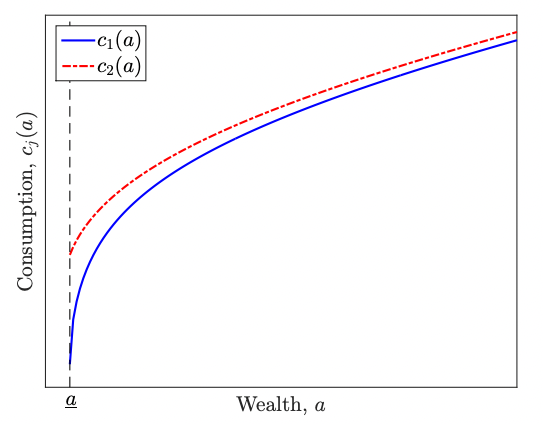
\includegraphics[width=.45\textwidth]{./figures/HACT_consumption}\qquad
	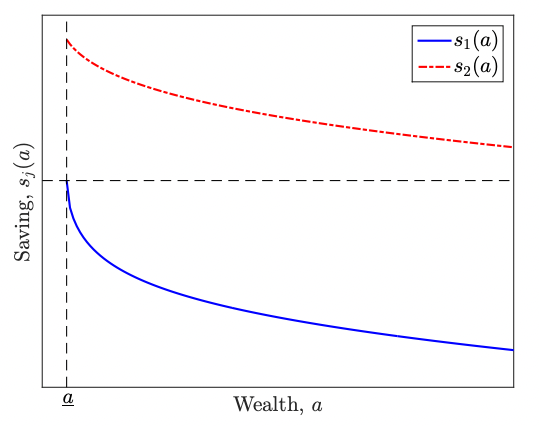
\includegraphics[width=.45\textwidth]{./figures/HACT_savings}
\end{frame}


%%%%%%%%%%%%%%%%%%%%%%%%%%  SLIDE   %%%%%%%%%%%%%%%%%%%%%%%%%%%%%%%%
\begin{frame}{Typical Stationary Distribution}
	\vspace{1cm}
	\centering
	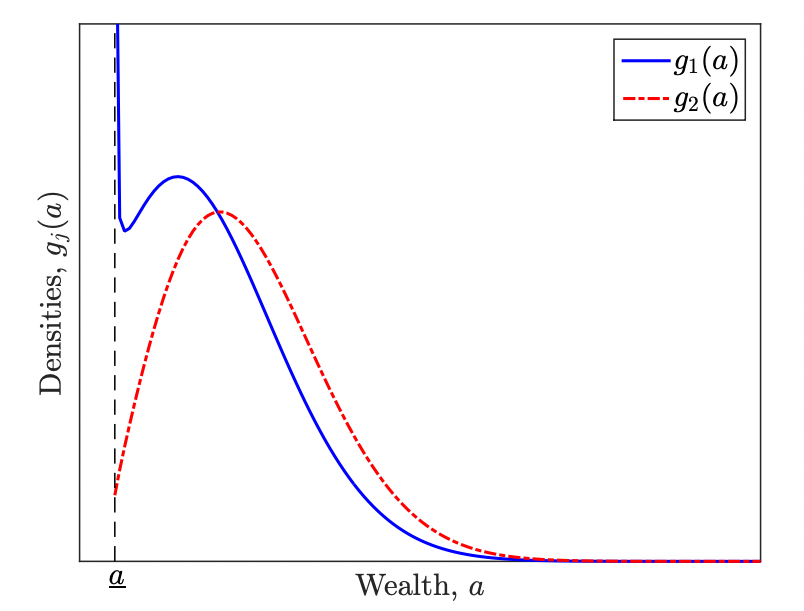
\includegraphics[width=.5\textwidth]{./figures/HACT_distribution}
\end{frame}


%%%%%%%%%%%%%%%%%%%%%%%%%%  SLIDE   %%%%%%%%%%%%%%%%%%%%%%%%%%%%%%%%
\begin{frame}{Household MPC}
\begin{center}
	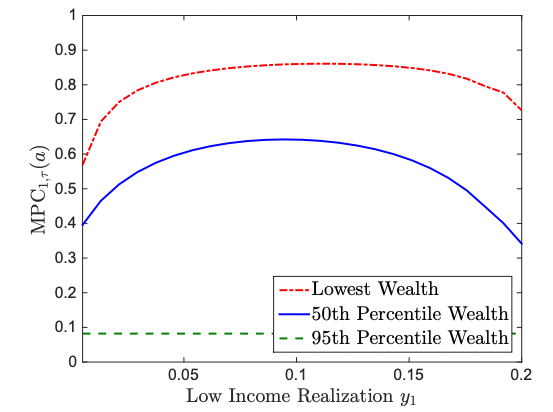
\includegraphics[width=0.5\textwidth]{./figures/HACT_MPC}
\end{center}
\end{frame}


%%%%%%%%%%%%%%%%%%%%%%%%%%  SLIDE   %%%%%%%%%%%%%%%%%%%%%%%%%%%%%%%%
\begin{frame}{General Equilibrium: Existence and Uniqueness}
	\begin{figure}[tph]
		\centering
		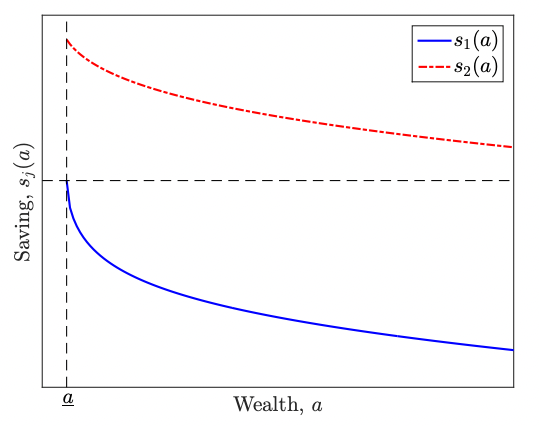
\includegraphics[width=.45\textwidth]{./figures/HACT_savings} \qquad 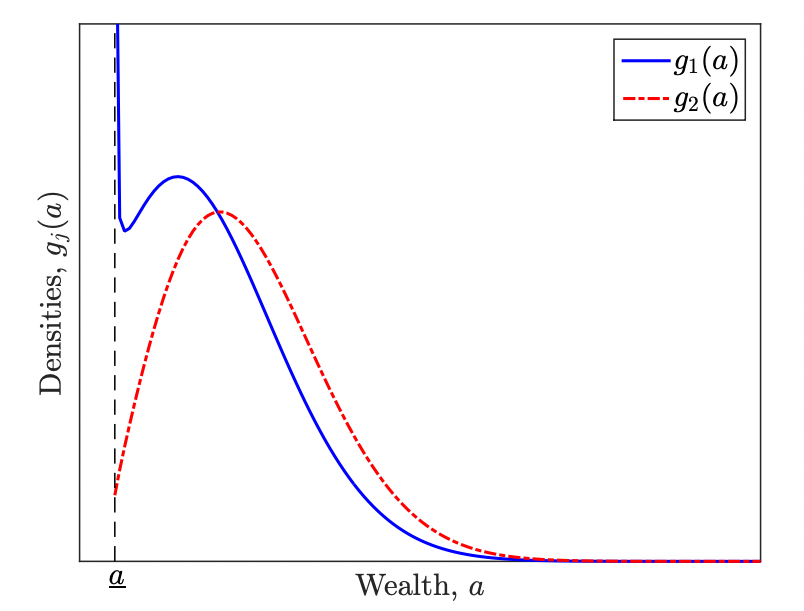
\includegraphics[width=.45\textwidth]{./figures/HACT_distribution}
	\end{figure}
\end{frame}


%%%%%%%%%%%%%%%%%%%%%%%%%%  SLIDE   %%%%%%%%%%%%%%%%%%%%%%%%%%%%%%%%
\begin{frame}{Increase in $r$ from $r_L$ to $r_H>r_L$}
	\begin{figure}[ht]
		\centering
		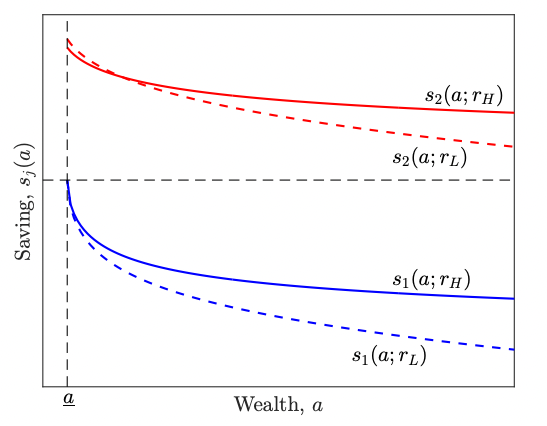
\includegraphics[width=.45\textwidth]{./figures/HACT_savings2} \qquad 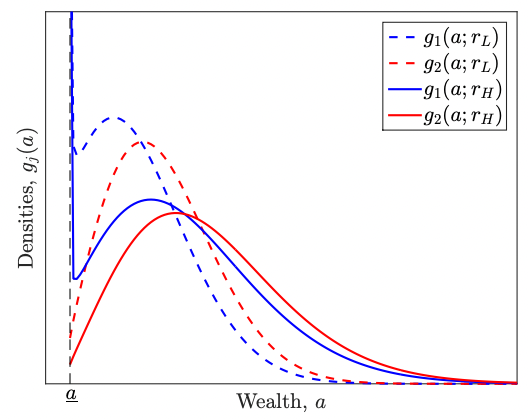
\includegraphics[width=.45\textwidth]{./figures/HACT_distribution2}
	\end{figure}
\end{frame}


%%%%%%%%%%%%%%%%%%%%%%%%%%  SLIDE   %%%%%%%%%%%%%%%%%%%%%%%%%%%%%%%%
\begin{frame}{Stationary Equilibrium}
\begin{figure}[tph]
	\centering
	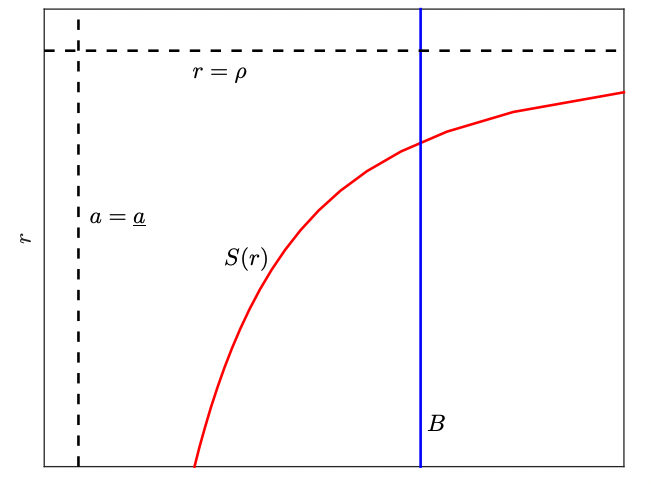
\includegraphics[width=0.45\textwidth]{./figures/HACT_existence}
\end{figure}

\vspace{-4mm}
{\small $$\mbox{Asset Supply} \quad S(r) = \int_{\ushort{a}}^\infty a g_1(a;r)da + \int_{\ushort{a}}^\infty a g_2(a;r)da $$}

\pause
\vspace{2mm}
{\color{blue}\textbf{Proposition}}: a stationary equilibrium exists (also unique!)
\end{frame}


%%%%%%%%%%%%%%%%%%%%%%%%%%  SLIDE   %%%%%%%%%%%%%%%%%%%%%%%%%%%%%%%%
\begin{frame}{Extension: Diffusion Income Process}
\begin{figure}[ht]
	\centering
	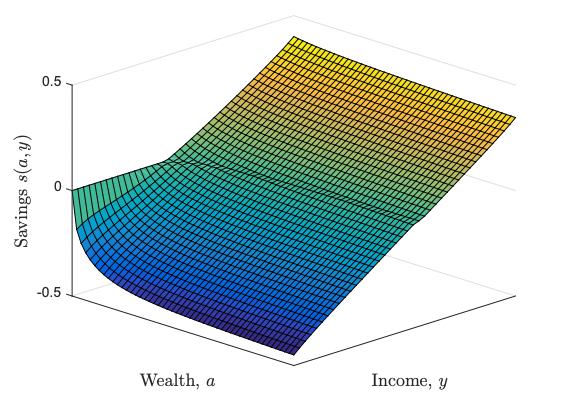
\includegraphics[width=.45\textwidth]{./figures/HACT_diffusion_savings} \qquad 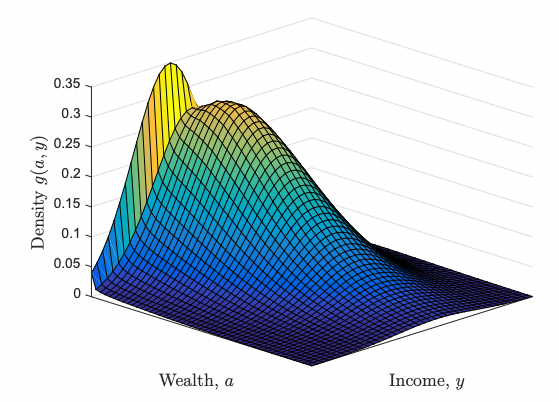
\includegraphics[width=.45\textwidth]{./figures/HACT_diffusion_distribution}
\end{figure}
\end{frame}


\end{document}

%%%%%%%%%%%%%%%%%%%%%%%%%%  SLIDE   %%%%%%%%%%%%%%%%%%%%%%%%%%%%%%%%
\begin{transitionframe}
	{\color{white} \huge \textbf{Part 3: Appendix Slides from Ben Moll} \vspace{2mm}}
\end{transitionframe}


%%%%%%%%%%%%%%%%%%%%%%%%%%  SLIDE   %%%%%%%%%%%%%%%%%%%%%%%%%%%%%%%%
\begin{frame}{Transition Dynamics}
	\bi
	\item Needed whenever initial condition $\neq$ stationary distribution
	\bigskip
	\item Equilibrium still coupled systems of HJB and KF equations...
	\bigskip
	\item ... but now \tr{time-dependent}: $v_j(a,\tr{t})$ and $g_j(a,\tr{t})$
	\bigskip
	\item See next slides for equations
	\bigskip
	\item Difficulty: the two PDEs run in opposite directions in time
	\bi
	\medskip
	\item HJB looks forward, runs backwards from terminal condition
	\medskip
	\item KF looks backward, runs forward from initial condition
	\ei
	\ei
\end{frame}


%%%%%%%%%%%%%%%%%%%%%%%%%%  SLIDE   %%%%%%%%%%%%%%%%%%%%%%%%%%%%%%%%
\begin{frame}{Transition Dynamics}
	\vspace{-5mm}
	{\small 
		\begin{align}
			\tag{EQ} B = & \int_{\ushort{a}}^\infty a g_1(a,t)da + \int_{\ushort{a}}^\infty a g_2(a,t)da\\[2ex]
			\tag{HJB}\begin{split}
				\rho v_j(a,t) =& \max_c \ u(c) + \partial_a v_j(a,t)(y_j + r(t) a - c)\\
				& + \lambda_j(v_{-j}(a,t) - v_j(a,t)) + \partial_t v_j(a,t), 
			\end{split}\\[2ex]
			\tag{KF}\partial_t g_j(a,t) =& - \partial_a[s_j(a,t)g_j(a,t)] - \lambda_j g_j(a,t) + \lambda_{-j} g_{-j}(a,t),\\[1ex]
			\notag s_j(a,t) =& y_j + r(t) a - c_j(a,t), \quad c_j(a,t) = (u')^{-1}(\partial_a v_j(a,t)),\\[1ex]
			\notag & \int_{\ushort{a}}^\infty (g_1(a,t) + g_2(a,t))da = 1, \quad g_1,g_2 \geq 0
	\end{align}}
	\vspace{-4mm}
	\begin{itemize}
		\item Given initial condition $g_{j,0}(a)$, the two PDEs (HJB) and (KF) together with (EQ) fully characterize equilibrium.
		\medskip
		\item Notation: for any function $f$, $\partial_x f$ means $\frac{\partial f}{\partial x}$
	\end{itemize}
\end{frame}




%%%%%%%%%%%%%%%%%%%%%%%%%%  SLIDE   %%%%%%%%%%%%%%%%%%%%%%%%%%%%%%%%
\begin{frame}{Plan}
	\begin{itemize}
		\item  \tr{New theoretical results:}
		\be
		\medskip
		\item analytics: consumption, saving, MPCs of the poor
		\bigskip
		\item closed-form for wealth distribution with 2 income types
		\bigskip
		\item unique stationary equilibrium if IES $\geq 1$ (sufficient condition)
		\bigskip
		\item ``soft" borrowing constraints
		\ee
		\medskip
		Note: for 1., 2. and 4. analyze \tr{partial equilibrium} with $r<\rho$
		\bigskip
		\medskip
		\item \tr{Computational algorithm:}
		\bi
		\bigskip
		\item problems with non-convexities
		\bigskip
		\item transition dynamics
		\ei
	\end{itemize}
\end{frame}





%\begin{frame}{Result 1: Consumption, Saving Behavior of the Poor}
%\vspace{-3mm}
%Consumption/saving behavior near borrowing constraint depends on:
%\begin{enumerate}
%\medskip
%\item tightness of constraint
%\medskip
%\item properties of $u$ as $c\rightarrow 0$
%\end{enumerate}
%\pause
%\bigskip
%\tr{Assumption 1:}\newline \emph{As $a \rightarrow \ushort{a}$, coefficient of absolute risk aversion $R(c) := -u''(c)/u'(c)$ remains finite}
%$$ - \frac{u''(y_1 +  r\ushort{a})}{u'(y_1 + r\ushort{a})}<\infty$$
%\vspace{-3mm}
%\bi 
%\item will show: A1 $\Rightarrow$ borrowing constraint ``matters" (in fact, it's an $\Leftrightarrow$)
%\medskip
%\ei
%\pause
%How to read A1?
%\bi
%\medskip
%\item for ``standard" $u$ functions (e.g. CRRA): equivalent to $\ushort{a}>-y_1/r$
%\medskip
%\item but weaker: \tr{only violated if both} $\ushort{a}=-y_1/r$ \tr{and} $-\tfrac{u''(0)}{u'(0)}=\infty$
%%IN THIS CASE BORROWING CONSTRAINT IS UNINTERESTING, IN ALL OTHER CASES IT WILL BE
%\medskip
%\item e.g. if $u'(c)= e^{-\theta c}$: A1 holds \& constraint matters even if $\ushort{a}=-\tfrac{y_1}{r}$
%\ei
%\end{frame}



%%%%%%%%%%%%%%%%%%%%%%%%%%  SLIDE   %%%%%%%%%%%%%%%%%%%%%%%%%%%%%%%%
\begin{transitionframe}
	{\color{white} \Huge \textbf{Theoretical Results} \vspace{2mm}}
\end{transitionframe}


%%%%%%%%%%%%%%%%%%%%%%%%%%  SLIDE   %%%%%%%%%%%%%%%%%%%%%%%%%%%%%%%%
\begin{frame}{Result 1: Consumption, Saving Behavior of the Poor}
	Consumption/saving behavior near borrowing constraint depends on:
	\begin{enumerate}
		\item tightness of constraint
		\item properties of $u$ as $c\rightarrow 0$
	\end{enumerate}
	\pause
	\medskip
	\tr{Assumption 1:}\newline \emph{As $a \rightarrow \ushort{a}$, coefficient of absolute risk aversion $R(c) := -u''(c)/u'(c)$ remains finite}
	$$ - \frac{u''(y_1 +  r\ushort{a})}{u'(y_1 + r\ushort{a})}<\infty$$
	\vspace{-3mm}
	\bi 
	\item will show: A1 $\Rightarrow$ borrowing constraint ``matters" (in fact, it's an $\Leftrightarrow$)
	\medskip
	\ei
	\pause
	How to read A1?
	\bi
	\item ``standard" utility functions, e.g. CRRA, satisfy $-\tfrac{u''(0)}{u'(0)}=\infty$
	\item hence for standard utility functions A1 equivalent to $\ushort{a}>-y_1/r$, i.e. constraint matters if it is tighter than ``natural borrowing constraint"
	\item  but weaker: e.g. if $u'(c)= e^{-\theta c}$, constraint matters even if $\ushort{a}=-\tfrac{y_1}{r}$
	%\item for ``standard" $u$ functions (e.g. CRRA): equivalent to $\ushort{a}>-y_1/r$
	%\medskip
	%\item but weaker: \tr{only violated if both} $\ushort{a}=-y_1/r$ \tr{and} $-\tfrac{u''(0)}{u'(0)}=\infty$
	%%IN THIS CASE BORROWING CONSTRAINT IS UNINTERESTING, IN ALL OTHER CASES IT WILL BE
	%\medskip
	%\item e.g. if $u'(c)= e^{-\theta c}$: A1 holds \& constraint matters even if $\ushort{a}=-\tfrac{y_1}{r}$
	\ei
\end{frame}



%%%%%%%%%%%%%%%%%%%%%%%%%%  SLIDE   %%%%%%%%%%%%%%%%%%%%%%%%%%%%%%%%
\begin{frame}{Result 1: Consumption, Saving Behavior of the Poor}
	Rough version of Proposition: under A1 policy functions look like this\\
	\vspace{1cm}
	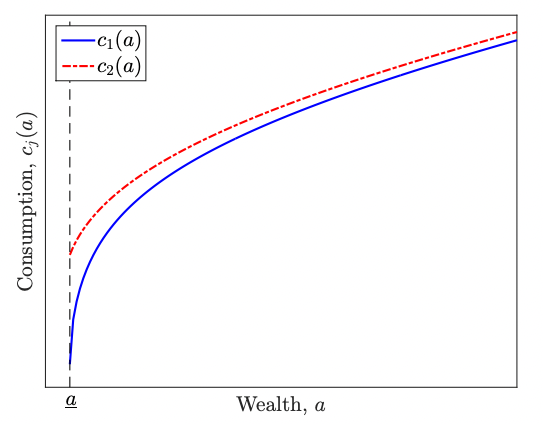
\includegraphics[width=.45\textwidth]{./figures/HACT_consumption}\qquad
	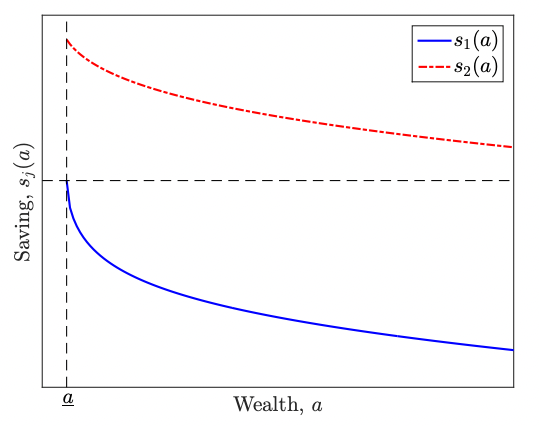
\includegraphics[width=.45\textwidth]{./figures/HACT_savings}
\end{frame}


%%%%%%%%%%%%%%%%%%%%%%%%%%  SLIDE   %%%%%%%%%%%%%%%%%%%%%%%%%%%%%%%%
\begin{frame}{Result 1: Consumption, Saving Behavior of the Poor}\label{prop:sav}
	\tr{\textbf{Proposition:}} Assume $r<\rho, y_1<y_2$ and that A1 holds.\\ Then saving and consumption policy functions close to $a=\ushort{a}$ satisfy
	\begin{align*}
		s_1(a) &\sim -  \sqrt{2\nu_1}\tr{\sqrt{a - \ushort{a}}}\\[1.2ex]
		c_1(a) &\sim y_1 + r a + \sqrt{2\nu_1}\tr{\sqrt{a - \ushort{a}}}\\[1.2ex]
		c_1'(a) &\sim r + \frac{1}{2} \sqrt{\frac{\nu_1}{2\tr{(a - \ushort{a})}}}
	\end{align*}
	where $\nu_1=$ constant that depends on $r,\rho,\lambda_1,\lambda_2$ etc -- see next slide
	\\
	\bigskip
	{\footnotesize Note: ``$f(a)\sim g(a)$" means $\lim_{a \rightarrow \ushort{a}}f(a)/g(a)=1$, ``$f$ behaves like $g$ close to $\ushort{a}$"}
\end{frame}



%%%%%%%%%%%%%%%%%%%%%%%%%%  SLIDE   %%%%%%%%%%%%%%%%%%%%%%%%%%%%%%%%
\begin{frame}{Result 1: Consumption, Saving Behavior of the Poor}
	\tr{\textbf{Corollary:}} The wealth of worker who keeps $y_1$ converges to borrowing constraint {\tr{in finite time}} at speed governed by $\tr{\nu_1}$:
	%\begin{align*}
	%a(t) - \ushort{a} &\sim \frac{\tr{\nu_1}}{2}\left(\tb{T}-t\right)^2 , \quad 0 \leq t\leq \tb{T}, \quad \mbox{where}\\
	%\tb{T} & := \tb{\mbox{``hitting time"}} = \tb{\sqrt{\tfrac{2(a_0 - \ushort{a})}{\nu_1}}}
	%\end{align*}
	\begin{align*}
		a(t) - \ushort{a} &\sim \frac{\tr{\nu_1}}{2}\left(\tb{T}-t\right)^2, \quad \tb{T} := \tb{\mbox{``hitting time"}} = \tb{\sqrt{\tfrac{2(a_0 - \ushort{a})}{\nu_1}}}, \quad 0 \leq t\leq \tb{T}
	\end{align*}
	Proof: integrate $\dot{a}(t) = - \sqrt{2\tr{\nu_1}}\sqrt{a(t) - \ushort{a}}$\\
	\bigskip
	\pause
	And have analytic solution for speed
	\begin{align*}
		{\tr{\nu_1}} &= \frac{(\rho - r)u'(\ushort{c}_{1}) + \lambda_1 (u'(\ushort{c}_{1}) - u'(\ushort{c}_{2}))}{-u''(\ushort{c}_{1})} \\
		&\approx \tr{(\rho-r)\textrm{IES}(\ushort{c}_1)\ushort{c}_1 + \lambda_1(\ushort{c}_2 - \ushort{c}_1)}
	\end{align*}
\end{frame}




%%%%%%%%%%%%%%%%%%%%%%%%%%  SLIDE   %%%%%%%%%%%%%%%%%%%%%%%%%%%%%%%%
\begin{frame}{Intuition for Result 1: Two Special Cases}
	\bi
	\item What's the role of A1? And why the square root?
	\bigskip
	\item Explain using two special cases with \tr{analytic solution}
	\bigskip
	\item Both cases: \tr{no income uncertainty}
	\ei
\end{frame}


%%%%%%%%%%%%%%%%%%%%%%%%%%  SLIDE   %%%%%%%%%%%%%%%%%%%%%%%%%%%%%%%%
\begin{frame}{Intuition for Result 1: Two Special Cases}
	\bi
	\item Special case 1: A1 holds, \tr{hit} constraint
	\ei
	\centering
	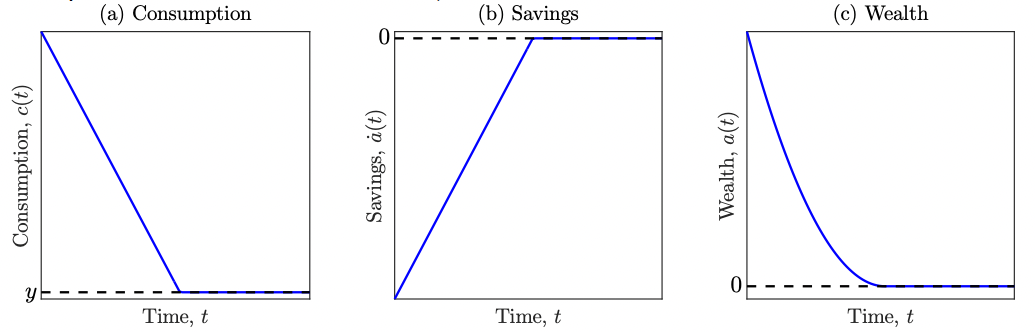
\includegraphics[width=.6\textwidth]{./figures/HACT_example1}
	\bi
	\item Special case 2: A1 violated, \tr{approach} constraint \tr{asymptotically}
	\medskip
	\ei
	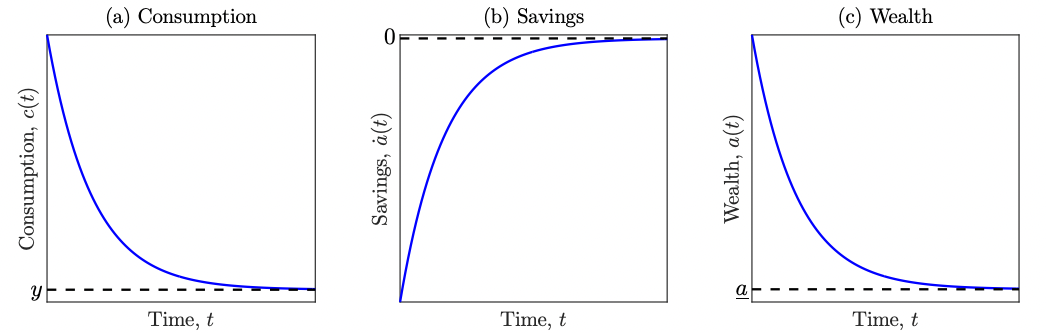
\includegraphics[width=.6\textwidth]{./figures/HACT_example2}
\end{frame}


%%%%%%%%%%%%%%%%%%%%%%%%%%  SLIDE   %%%%%%%%%%%%%%%%%%%%%%%%%%%%%%%%
\begin{frame}{}
	\vspace{4mm}
	Special case 1: \tr{hit} constraint
	\bi
	\smallskip
	\item exponential utility $u'(c) = e^{-\theta c}$, tight constraint
	$$\dot{c} = \frac{1}{\theta}(r-\rho), \qquad \dot{a} = y + ra - c, \qquad a \geq 0$$
	\item satisfies A1: $-\frac{u''(y)}{u'(y)} = \theta <\infty$. \uncover<2->{Solution:
		\begin{align*}
			c(t) &= y + \tr{\nu}(\tb{T}-t), \quad a(t) = \frac{\tr{\nu}}{2}(\tb{T}-t)^2, \quad \tr{\nu := \tfrac{\rho-r}{\theta}}
			%\\
			%&\Rightarrow \quad c(a) = y + \sqrt{2 \nu a}
		\end{align*}
	}
	%\item<2->{Solution:}
	\ei
	\vspace{-3mm}
	Special case 2: only \tr{approach} constraint \tr{asymptotically}
	\bi
	\medskip
	\item CRRA utility $u'(c) = c^{-\gamma}$, loose constraint 
	$$\frac{\dot{c}}{c} = \frac{1}{\gamma}(r-\rho), \qquad \dot{a} = y +  ra - c, \qquad a \geq \tr{\ushort{a} =-\frac{y}{r}}$$
	\item violates A1: $-\frac{u''(y +  ra)}{u'(y + ra)} \rightarrow \infty$ as $a\rightarrow \ushort{a}$. \uncover<3->{Solution:
		$$c(t) = y + (r + \tr{\eta})a(t), \quad a(t) - \ushort{a} = (a_0 - \ushort{a}) e^{-\tr{\eta} t}, \quad \tr{\eta:=\tfrac{\rho-r}{\gamma}}  $$ }
	\ei
\end{frame}


%%%%%%%%%%%%%%%%%%%%%%%%%%  SLIDE   %%%%%%%%%%%%%%%%%%%%%%%%%%%%%%%%
\begin{frame}{Intuition for Result 1: Two Special Cases}
	\bi
	\item Special case 1: A1 holds, \tr{hit} constraint
	\ei
	\centering
	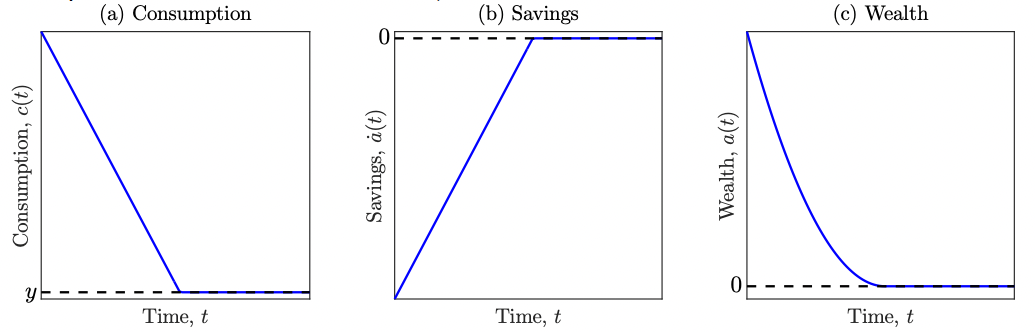
\includegraphics[width=.6\textwidth]{./figures/HACT_example1}
	\bi
	\item Special case 2: A1 violated, \tr{approach} constraint \tr{asymptotically}
	\medskip
	\ei
	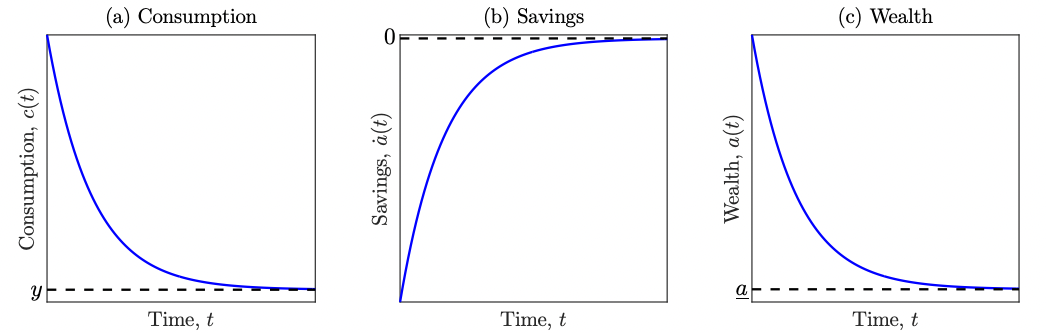
\includegraphics[width=.6\textwidth]{./figures/HACT_example2}
\end{frame}

%\begin{frame}{Special Case 1: \tr{Exponential utility} $u'(c)=e^{-\theta c}$}
%\vspace{-6mm}
%\begin{align*}
%\dot{c} = \frac{1}{\theta}(r-\rho), \qquad \dot{a} = y + ra - c, \qquad a \geq 0
%\end{align*}
%\pause
%\vspace{-3mm}
%\bi
%\item Solution: {\scriptsize(2nd line assumes $r=0$, case $r\neq 0$ similar)}
%\begin{equation}\tag{$\ast$}\label{eq:XYZ}
%\begin{split}
%c(t) &= y + \tr{\nu}(\tb{T}-t), \quad \tr{\nu := \tfrac{\rho-r}{\theta}}\\
%a(t) &= \frac{\tr{\nu}}{2}(\tb{T}-t)^2
%\end{split}
%\end{equation}
%\ei
%\hspace*{-1.2cm} \includegraphics[width=.95\textwidth]{../../../../../Papers/Heterogeneity_Macro/graphs_not_numerical/fig_xavier_exp.eps}
%\bi
%\item And note: \eqref{eq:XYZ} implies $c(a) = y + \sqrt{2 \nu a}$
%\ei
%\end{frame}

%
%\begin{frame}{Special Case 2: \tr{CRRA utility} $u'(c)=c^{-\gamma}$}
%\vspace{-7mm}
%\begin{align*}
%\frac{\dot{c}}{c} = \frac{1}{\gamma}(r-\rho), \qquad \dot{a} = y +  ra - c, \qquad a \geq \tr{\ushort{a} =-\frac{y}{r}}
%\end{align*}
%\bi
%\item Note this violates Assumption 1: $-\frac{u''(y +  ra)}{u'(y + ra)} \rightarrow \infty$ as $a\rightarrow \ushort{a}$
%\pause
%\bigskip
%\item Solution:
%\vspace{-3mm}
%\begin{align*}
%\dot{a}(t) - \ushort{a} &= -\tr{\eta} (a(t) - \ushort{a}) \quad \mbox{where} \quad \tr{\eta:=\frac{\rho-r}{\gamma}}\\
%\Rightarrow \quad a(t) - \ushort{a} &= (a_0 - \ushort{a}) e^{-\tr{\eta} t} \quad \Rightarrow \quad \mbox{\tr{never hit constraint!}}
%\end{align*}
%\ei
%\medskip
%\hspace*{-1.2cm} \includegraphics[width=.95\textwidth]{../../../../../Papers/Heterogeneity_Macro/graphs_not_numerical/fig_xavier_CRRA2.eps}
%\end{frame}




%%%%%%%%%%%%%%%%%%%%%%%%%%  SLIDE   %%%%%%%%%%%%%%%%%%%%%%%%%%%%%%%%
\begin{frame}{Consumption, Saving Behavior of the Rich}
	\bi
	\item Skip this today. See paper.
	\ei
\end{frame}



%%%%%%%%%%%%%%%%%%%%%%%%%%  SLIDE   %%%%%%%%%%%%%%%%%%%%%%%%%%%%%%%%
\begin{frame}{Marginal Propensities to Consume and Save}
	\bi
	\item So far: have characterized $c'_j(a)$ \tr{$\neq$ MPC over discrete time interval}
	\medskip
	\pause
	\item \textbf{\tr{Definition:}} The MPC over a time period $\tau$ is given by
	\begin{align*}
		\textrm{MPC}_{j,\tau}(a) &=  C_{j,\tau}'(a), \quad \mbox{where}\\
		C_{j,\tau}(a) &= \mathbb{E}\left[\int_0^\tau c_{j}(a_t)dt \vert a_0 = a,y_0 = y_j \right]
	\end{align*}
	\pause
	\item \textbf{\tr{Lemma:}} If \tr{$\tau$ sufficiently small} so that no income switches, then
	$$\textrm{MPC}_{1,\tau}(a) \sim \min\{\tau c_1'(a),1 + \tau r\}$$
	Note: $\textrm{MPC}_{1,\tau}(a)$ bounded above even though $c_1'(a)\rightarrow \infty$ as $a \downarrow \ushort{a}$
	\pause
	\bigskip
	\item  If new income draws before $\tau$, no more analytic solution
	\bigskip
	\item But straightforward computation using \textbf{\tr{Feynman-Kac formula}}
	\ei
\end{frame}




%\begin{frame}{Using the Formula for $\nu_1$ to Better Understand MPCs}
%\vspace{-3mm}
%\bi
%\item Consider dependence of low-income type's $\textrm{MPC}_{1,\tau}(a)$ on $y_1$
%\pause
%\bigskip
%\begin{center}
%\includegraphics[width=0.45\textwidth]{../../../../../Papers/Heterogeneity_Macro/code/partial_eq_compstatics/figMPC2b.eps}
%\end{center}
%\vspace{-3mm}
%\item \tr{Why hump-shaped?!?}
%\pause
%\bigskip
%\item Answer: $\nu_1 \approx (\rho-r)\textrm{IES}(\ushort{c}_1)\ushort{c}_1 + \lambda_1(\ushort{c}_2 - \ushort{c}_1)$. With CRRA
%$$\nu_1 \approx (\rho-r)\frac{\tr{\ushort{c}_1}}{\gamma} + \lambda_1(\ushort{c}_2 - \tr{\ushort{c}_1}), \qquad \tr{\ushort{c}_1} = \tr{y_1} + r \ushort{a}$$
%Can see: increase in $\tr{y_1}$ has two \tr{offsetting effects}
%\ei
%\end{frame}


%%%%%%%%%%%%%%%%%%%%%%%%%%  SLIDE   %%%%%%%%%%%%%%%%%%%%%%%%%%%%%%%%
\begin{frame}{Using the Formula for $\nu_1$ to Better Understand MPCs}
	\bi
	\item Consider dependence of low-income type's $\textrm{MPC}_{1,\tau}(a)$ on $y_1$
	\pause
	\begin{center}
		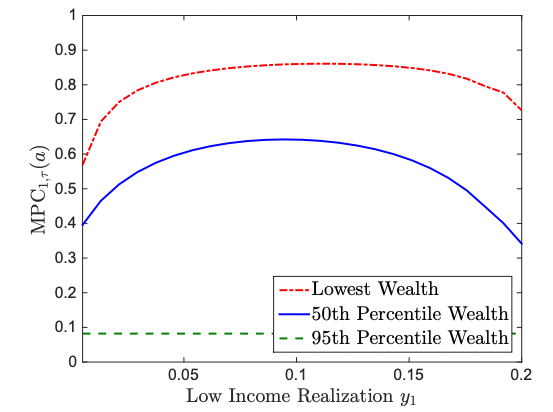
\includegraphics[width=0.4\textwidth]{./figures/HACT_MPC}
	\end{center}
	\vspace{-1mm}
	\item \tr{Why hump-shaped?!?} \pause Answer: $\textrm{MPC}_{1,\tau}(a)$ proportional to
	\begin{align*}
		c_1'(a) &\sim r + \frac{1}{2} \sqrt{\frac{{\tr{\nu_1}}}{2(a - \ushort{a})}}, \quad \tr{\nu_1} \approx (\rho-r)\frac{1}{\gamma} \tr{\ushort{c}_1}+ \lambda_1(\ushort{c}_2 - \tr{\ushort{c}_1})\\
		&\mbox{and note that} \ \tr{\ushort{c}_1} = \tr{y_1} + r \ushort{a}
	\end{align*}
	\item Can see: increase in $\tr{y_1}$ has two \tr{offsetting effects}
	\ei
\end{frame}







\begin{frame}{Result 2: Stationary Wealth Distribution}
	\begin{itemize}
		\item Recall equation for stationary distribution
		\begin{equation}\tag{KF}\label{eq:KF2}0 = - \frac{d}{da}[s_j(a)g_j(a)] - \lambda_j g_j(a) + \lambda_{-j} g_{-j}(a)\end{equation}
		\item \textbf{\tr{Lemma:}} the solution to \eqref{eq:KF2} is
		\begin{align*}
			g_i(a) = \frac{\kappa_j}{s_j(a)}\exp\left(-\int_{\ushort{a}}^a \left(\frac{\lambda_1}{s_1(x)} + \frac{\lambda_2}{s_2(x)} dx\right)\right)
		\end{align*}
		with $\kappa_1,\kappa_2$ pinned down by $g_j$'s integrating to one
		\bigskip
		\item \tr{Features of wealth distribution:}
		\bi
		\medskip
		\item Dirac  {\tr{point mass}} of type $y_1$ individuals at constraint $G_1(\ushort{a})>0$
		\medskip
		\item \tr{thin right tail}: $g(a) \sim \xi(a_{\max} - a)^{\lambda_2/\zeta_2 - 1}$, i.e. not Pareto 
		\medskip
		\item see paper for more
		\ei
		\bigskip
		\item Later in paper: extension with Pareto tail (Benhabib-Bisin-Zhu)
	\end{itemize}
\end{frame}






%%%%%%%%%%%%%%%%%%%%%%%%%%  SLIDE   %%%%%%%%%%%%%%%%%%%%%%%%%%%%%%%%
\begin{frame}{Result 2: Stationary Wealth Distribution}
	\vspace{1cm}
	\centering
	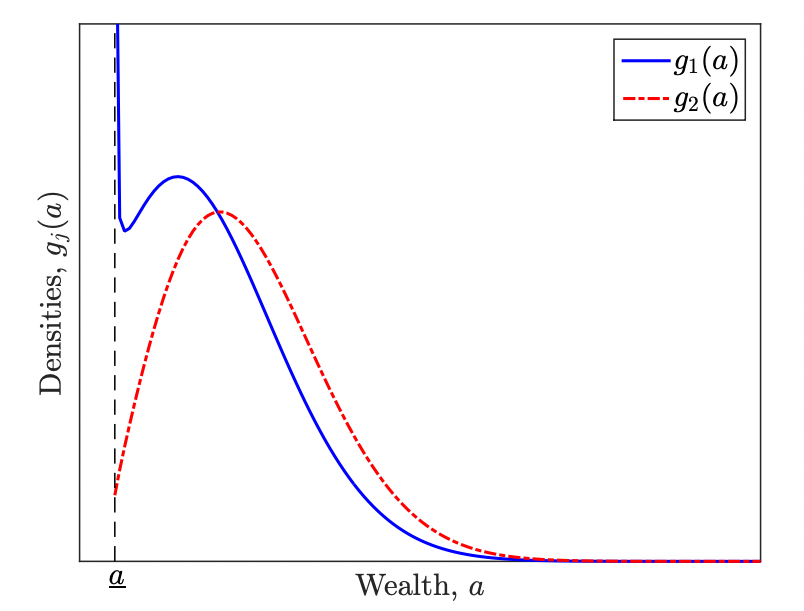
\includegraphics[width=.5\textwidth]{./figures/HACT_distribution}
	
	Note: in numerical solution, Dirac mass = finite spike in density
\end{frame}





%%%%%%%%%%%%%%%%%%%%%%%%%%  SLIDE   %%%%%%%%%%%%%%%%%%%%%%%%%%%%%%%%
\begin{frame}{General Equilibrium: Existence and Uniqueness}
	\begin{figure}[tph]
		\centering
		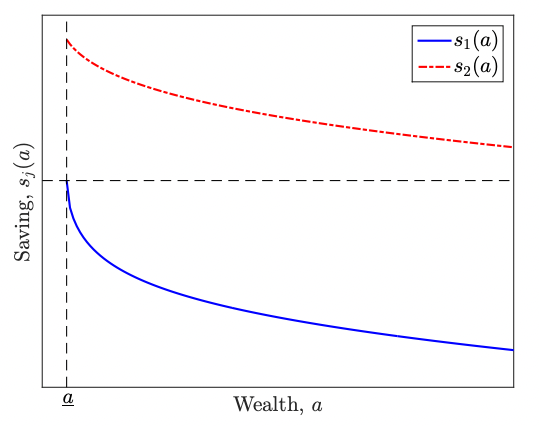
\includegraphics[width=.45\textwidth]{./figures/HACT_savings} \qquad 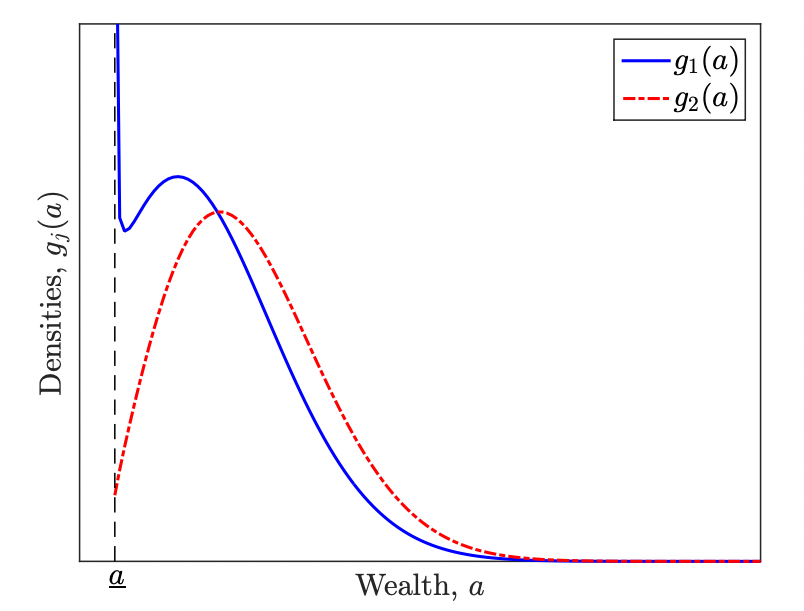
\includegraphics[width=.45\textwidth]{./figures/HACT_distribution}
	\end{figure}
\end{frame}


%%%%%%%%%%%%%%%%%%%%%%%%%%  SLIDE   %%%%%%%%%%%%%%%%%%%%%%%%%%%%%%%%
\begin{frame}{Increase in $r$ from $r_L$ to $r_H>r_L$}
	\begin{figure}[ht]
		\centering
		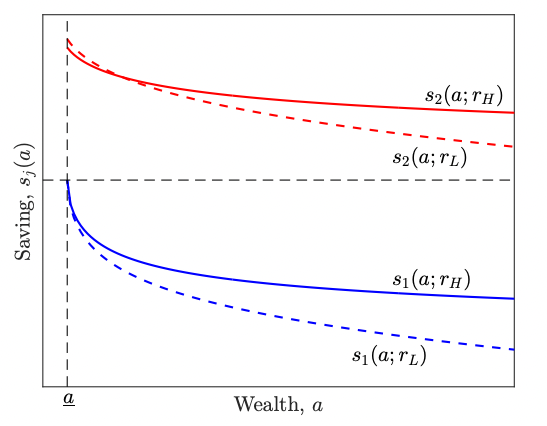
\includegraphics[width=.45\textwidth]{./figures/HACT_savings2} \qquad 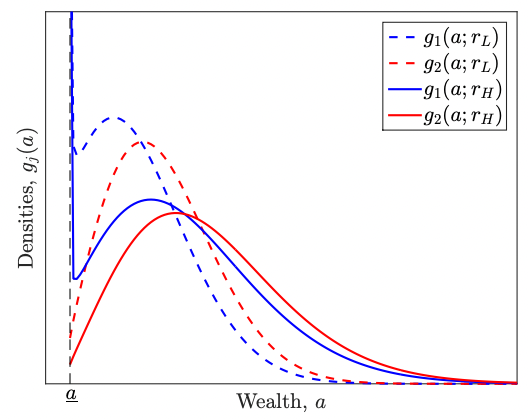
\includegraphics[width=.45\textwidth]{./figures/HACT_distribution2}
	\end{figure}
\end{frame}

%%%%%%%%%%%%%%%%%%%%%%%%%%  SLIDE   %%%%%%%%%%%%%%%%%%%%%%%%%%%%%%%%
\begin{frame}{Stationary Equilibrium}
	\begin{figure}[tph]
		\centering
		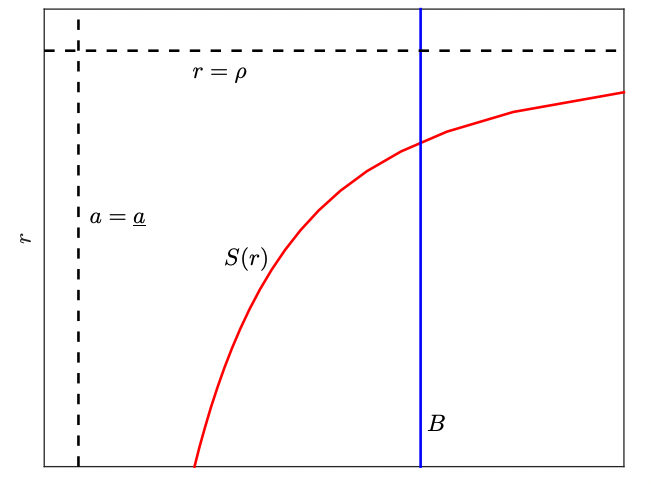
\includegraphics[width=0.45\textwidth]{./figures/HACT_existence}
	\end{figure}
	\vspace{-4mm}
	{\small $$\mbox{Asset Supply} \quad S(r) = \int_{\ushort{a}}^\infty a g_1(a;r)da + \int_{\ushort{a}}^\infty a g_2(a;r)da $$}
	%\vspace{-2mm}
	\pause
	\begin{itemize}
		\item \tr{\textbf{Proposition:}} a stationary equilibrium exists
	\end{itemize}
\end{frame}


%%%%%%%%%%%%%%%%%%%%%%%%%%  SLIDE   %%%%%%%%%%%%%%%%%%%%%%%%%%%%%%%%
\begin{frame}{Result 3: Uniqueness of Stationary Equilibrium}
	\tr{\textbf{Proposition:}} Assume that the IES is weakly greater than one
	$$\textrm{IES}(c):=-\frac{u'(c)}{u''(c)c} \geq 1 \quad \mbox{for all} \ c \geq 0,$$
	and that there is no borrowing $a \geq 0$. Then:
	\begin{enumerate}
		\bigskip
		\item Individual consumption $c_j(a;r)$ is strictly \tr{de}creasing in $r$
		\bigskip
		\item Individual saving $s_j(a;r)$ is strictly \tr{in}creasing in $r$
		\bigskip
		\item $r \uparrow \Rightarrow$ CDF $G_j(a;r)$ \tr{shifts right} in FOSD sense
		\bigskip
		\item Aggregate saving $S(r)$ is strictly \tr{in}creasing $\Rightarrow$ \tr{\textbf{uniqueness}}
	\end{enumerate}
	\bigskip
	Note: holds for \tr{any} labor income process, not just two-state Poisson
\end{frame}


%%%%%%%%%%%%%%%%%%%%%%%%%%  SLIDE   %%%%%%%%%%%%%%%%%%%%%%%%%%%%%%%%
\begin{frame}{Uniqueness: Proof Sketch}
	\vspace{-4mm}
	\begin{itemize}
		\item Parts 2 to 4 direct consequences of part 1 ($c_j(a;r)$ \tr{de}creasing in $r$)
		\medskip
		%\pause
		%\item e.g. part 2: without borrowing $a \geq 0$, $s_j(a;r)$ trivially increasing in $r$ 
		%$$s_j(a;r) = y_j + r a - c_j(a;r) \quad \Rightarrow \quad \frac{\partial s_j(a;r)}{\partial r} = a - \frac{\partial c_j(a;r)}{\partial r} > 0 $$ 
		%\vspace{-3mm}
		\pause
		\item $\Rightarrow$ focus on part 1: builds on nice result by Olivi (2017) who decomposes $\partial c_j/\partial r$ into \tb{income} and \tr{substitution} effects
		\bigskip
		\pause
		\item \tr{\textbf{Lemma} (Olivi, 2017):} $c$ response to change in $r$ is
	\end{itemize}
	{\small 
		\begin{align*}
			&\frac{\partial c_j(a)}{\partial r} = \underbrace{\frac{1}{u''(c_0)}\mathbb{E}_0\int_0^T e^{-\int_0^t \xi_s ds} \tr{u'(c_t)}dt}_{\textrm{\tr{substitution effect}} < 0} +  \underbrace{\frac{1}{u''(c_0)}\mathbb{E}_0\int_0^T e^{-\int_0^t \xi_s ds} \tb{u''(c_t)a_t \partial_a c_t}dt}_{\textrm{\tb{income effect}} > 0}\\
			& \qquad \mbox{where} \ \xi_t := \rho - r + \partial_a c_t \mbox{ and } T:=\inf\{t \geq 0| a_t = 0\} = \mbox{time at which hit } 0
	\end{align*}}
	\pause
	\vspace{-4mm}
	\bi
	\item We show: $\mbox{IES}(c):=-\frac{\tr{u'(c)}}{\tb{u''(c)}c} \geq 1 \Rightarrow$ \tr{substitution effect dominates} \\
	$\Rightarrow$ $\partial c_j(a)/\partial r < 0$, i.e. consumption  \tr{de}creasing in $r$
	\ei
\end{frame}


%%%%%%%%%%%%%%%%%%%%%%%%%%  SLIDE   %%%%%%%%%%%%%%%%%%%%%%%%%%%%%%%%
\begin{frame}{Result 4: ``Soft" Borrowing Constraints}
	\vspace{-3mm}
	\bi
	\item Empirical wealth distributions:
	\be
	\medskip
	\item individuals with \tr{positive} wealth
	\medskip
	\item individuals with \tr{negative} wealth
	\medskip
	\item \tr{spike at} close to \tr{zero} net worth
	\ee
	\bigskip
	\item Does not square well with Aiyagari-Bewley-Huggett model
	\pause
	\bigskip
	\item Simple solution: \tr{``soft"} borrowing constraint = \tr{wedge} between borrowing and saving $r$
	\bigskip
	\item Paper: \tr{first theoretical characterization} of ``soft" constraint
	\bi
	\medskip
	\item square root formulas
	\medskip
	\item Dirac mass at zero net worth
	\ei
	\ei
\end{frame}








%%%%%%%%%%%%%%%%%%%%%%%%%%  SLIDE   %%%%%%%%%%%%%%%%%%%%%%%%%%%%%%%%
\begin{transitionframe}
	{\color{white} \Huge \textbf{Computations} \vspace{2mm}}
\end{transitionframe}




%%%%%%%%%%%%%%%%%%%%%%%%%%  SLIDE   %%%%%%%%%%%%%%%%%%%%%%%%%%%%%%%%
\begin{frame}{Computational Advantages relative to Discrete Time}
\begin{enumerate}
	\item \tr{Borrowing constraints} only show up \tr{in boundary conditions}
	\bi
	\item FOCs always hold with ``$=$"
	\ei
	
	\medskip
	\item \tr{``Tomorrow is today"}
	\bi
	\item FOCs are ``static", compute by hand: $c^{-\gamma}=v_a(a,y)$
	\ei
	%\bi
	%\item FOCs 
	%\medskip
	%\item expectations $\neq$ integrals
	%\ei
	
	\medskip
	\item \tr{Sparsity}
	\begin{itemize}
		\item solving Bellman, distribution = inverting matrix
		\item but matrices very sparse (``tridiagonal")
		\item reason: continuous time $\Rightarrow$ one step left or one step right
	\end{itemize}

	\medskip
	\item \tr{Two birds with one stone}
	\bi
	\item tight link between solving (HJB) and (KF) for distribution
	\item matrix in discrete (KF) is \tr{transpose} of matrix in discrete (HJB)
	\item reason: diff. operator in (KF) is \tr{adjoint} of operator in (HJB)
	\ei
\end{enumerate}
\end{frame}



\begin{frame}{Computational Advantages relative to Discrete Time}
	\begin{enumerate}
		\item \tr{Borrowing constraints} only show up \tr{in boundary conditions}
		\bi
		\item FOCs always hold with ``$=$"
		\ei
		\medskip
		\item \tr{``Tomorrow is today"}
		\bi
		\item FOCs are ``static", compute by hand: $c^{-\gamma}= v_j'(a)$
		\ei
		\medskip
		\item \tr{Sparsity}
		\begin{itemize}
			\item solving Bellman, distribution = inverting matrix
			\item but matrices very sparse (``tridiagonal")
			\item reason: continuous time $\Rightarrow$ one step left or one step right
		\end{itemize}
		\medskip
		\item \tr{Two birds with one stone}
		\bi
		\item tight link between solving (HJB) and (KF) for distribution
		\item matrix in discrete (KF) is \tr{transpose} of matrix in discrete (HJB)
		\item reason: diff. operator in (KF) is \tr{adjoint} of operator in (HJB)
		\ei
	\end{enumerate}
\end{frame}



\begin{frame}{Computations for Heterogeneous Agent Model}
	\begin{itemize}
		\item \tr{Hard part}: HJB equation
		\item \tr{Easy part}: KF equation. Once you solved HJB equation, get KF equation ``for free"
		\pause
		\item System to be solved
	\end{itemize}
	{\small \begin{align*}
			\rho v_1(a) &=  \max_c \ u(c) + v_1'(a)(y_1 + ra - c) + \lambda_1(v_2(a) - v_1(a))\\
			\rho v_2(a) &=  \max_c \ u(c) + v_2'(a)(y_2 + ra - c) + \lambda_2(v_1(a) - v_2(a))\\
			0 &= - \frac{d}{da}[s_1(a)g_1(a)] - \lambda_1 g_1(a) + \lambda_2 g_2(a)\\
			0 &= - \frac{d}{da}[s_2(a)g_2(a)] - \lambda_2 g_2(a) + \lambda_1 g_1(a)\\
			1 &= \int_{\ushort{a}}^\infty g_1(a)da + \int_{\ushort{a}}^\infty g_2(a)da\\
			B &= \int_{\ushort{a}}^\infty a g_1(a)da + \int_{\ushort{a}}^\infty a g_2(a)da := S(r)
	\end{align*}}
\end{frame}




\begin{frame}{Bird's Eye View of Algorithm for Stationary Equilibria}
	\bi
	\item Use \tr{finite difference method}
	\medskip
	\item Discretize state space $a_i,i=1,...,I$ with step size $\Delta a$
	$$v_j'(a_i) \approx \frac{v_{i+1,j}-v_{i,j}}{\Delta a} \quad \mbox{or} \quad  \frac{v_{i,j}-v_{i-1,j}}{\Delta a} $$
	$$\mbox{Denote} \quad \mathbf{v} = \left[\begin{matrix} v_1(a_{1}) \\ \vdots \\ v_2(a_{I}) \end{matrix}\right], \quad \mathbf{g} = \left[\begin{matrix} g_1(a_{1}) \\ \vdots \\  g_2(a_{I}) \end{matrix}\right], \quad \mbox{dimension} = 2I \times 1 $$
	\smallskip
	\item End product of FD method: system of \tr{sparse matrix equations}
	\begin{align*}
		\rho \mathbf{v} &= \mathbf{u}(\mathbf{v}) + \mathbf{A}(\mathbf{v};r)\mathbf{v}\\
		\mathbf{0} &= \mathbf{A}(\mathbf{v};r)^{\rm T}\mathbf{g}\\
		B &= S(\mathbf{g};r)
	\end{align*}
	which is easy to solve on computer
	\ei
\end{frame}


\begin{frame}{Visualization of $\mathbf{A}$ (output of \url{spy(A)} in Matlab)}
	\begin{figure}[ht]
		\centering
		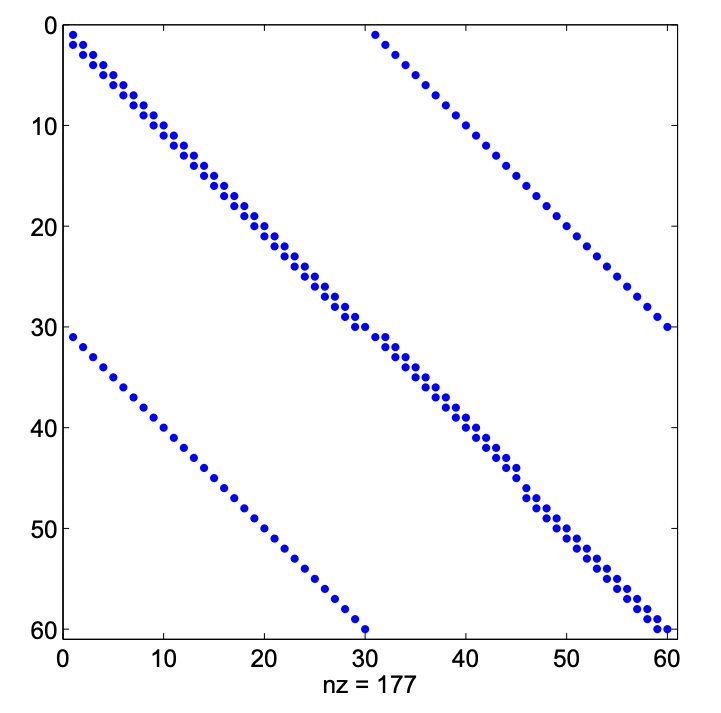
\includegraphics[width=.5\textwidth]{./figures/HACT_spyA}
	\end{figure}
\end{frame}



%\begin{frame}{HJB Equation: Barles-Souganidis}
%\vspace{-4mm}
%\bi
%\item There is a well-developed theory for numerical solution of HJB equation using finite difference methods
%\medskip
%\item Key paper:  Barles and Souganidis (1991), ``Convergence of approximation schemes for fully nonlinear second order equations
%%{\scriptsize \url{https://www.dropbox.com/s/vhw5qqrczw3dvw3/barles-souganidis.pdf?dl=0}}
%\medskip
%\item \tr{Result:} finite difference scheme ``converges" to unique viscosity solution under three conditions
%\begin{enumerate}
%\medskip
%\item monotonicity
%\medskip
%\item consistency
%\medskip
%\item stability
%\end{enumerate}
%\medskip
%\item Good reference: Tourin (2013), ``An Introduction to Finite Difference Methods for PDEs in Finance"
%\medskip
%\item Background on viscosity soln's: ``Viscosity Solutions for Dummies" {\scriptsize \url{http://www.princeton.edu/~moll/viscosity_slides.pdf}}
%\medskip
%\item Accuracy? \hyperlink{sli:accuracy}{\beamergotobutton{Two experiments}}, more in next revision -- suggestions?
%\ei
%\end{frame}






%\begin{frame}{HJB Equation}
%\begin{itemize}
%\item Discretized HJB equation is
%\begin{equation}\tag{HJBd}
%\rho \mathbf{v} = \mathbf{u(v)} + \mathbf{A}(\mathbf{v};r) \mathbf{v}
%\end{equation}
%\vspace{-5mm}
%\item $\mathbf{A}$ is $N \times N$ transition matrix
%\begin{itemize}
%\medskip
%\item here $N = 2 \times I$, $I$=number of wealth grid points
%\medskip
%\item $\mathbf{A}$ depends on $\mathbf{v}$ (nonlinear problem)
%%\medskip
%%\item solve using implicit scheme
%\end{itemize}
%\end{itemize}
%\end{frame}




%
%\begin{frame}{Computing the FK Equation}
%\vspace{-3mm}
%\begin{itemize}
%\item Equations to be solved
%{\small \begin{align*}
		%0 &= - \frac{d}{da}[s_1(a)g_1(a)] - \lambda_1 g_1(a) + \lambda_2 g_2(a)\\
		%0 &= - \frac{d}{da}[s_2(a)g_2(a)] - \lambda_2 g_2(a) + \lambda_1 g_1(a)
		%\end{align*}
		%with $1 = \int_{\ushort{a}}^\infty g_1(a)da + \int_{\ushort{a}}^\infty g_2(a)da$}
	%\pause
	%\smallskip
	%\item Actually, super easy: discretized version is simply
	%\begin{equation}\tag{KFd}0 = \mathbf{A}(\mathbf{v};r)^{\rm T} \mathbf{g}\end{equation}
	%\vspace{-5mm}
	%\begin{itemize}
	%\item \tr{eigenvalue problem}
	%\smallskip
	%\item get KF for free, one more reason for using implicit scheme
	%\end{itemize}
	%\medskip
	%\pause
	%\item Why transpose?
	%\begin{itemize}
	%\smallskip
	%\item operator in (HJB) is \tr{``adjoint"} of operator in (KF)
	%\smallskip
	%\item ``adjoint" = infinite-dimensional analogue of matrix transpose
	%\end{itemize}
	%\medskip
	%\item In principle, can use similar strategy in discrete time
	%\end{itemize}
	%\end{frame}
	
	
	
	
	
	%
	%\begin{frame}
	%\vspace{3.5cm}
	%\begin{center}
	%{\huge Transition Dynamics/MIT Shocks}
	%\end{center}
	%\end{frame}


\begin{frame}{Transition Dynamics: Intuition in Growth Model}
\bi
\item Next two slides: intuition for algorithm in rep agent growth model
\medskip
\item In three slides: solve Huggett model in exactly analogous fashion
\medskip
\item Equilibrium in growth model is solution to:
\begin{align*}
	\frac{\dot{C}(t)}{C(t)} &= \frac{1}{\gamma}(r(t) - \rho)\\[0.5ex]
	\dot{K}(t) &= w(t) + r(t)K(t) - C(t)\\[0.5ex]
	w(t) &= (1-\alpha) K(t)^\alpha, \quad r(t) = \alpha K(t)^{\alpha-1}\\[0.5ex]
	K(0) &= K_0, \quad \lim_{T\rightarrow \infty} C(T) = C_{\infty}
\end{align*}
\item For numerical solution, solve on $[0,T]$ for large $T$ with $C(T)=C_{\infty}$ 
\medskip
\item Define $w(r) = (1-\alpha) (\alpha/r)^{\frac{\alpha}{1-\alpha}} \Rightarrow$ only one price, $r(t)$
\ei
\end{frame}


\begin{frame}{Transition Dynamics: Intuition in Growth Model}
Equilibrium is therefore solution to
\begin{align}
	\label{eq:1}\frac{\dot{C}(t)}{C(t)} &= \frac{1}{\gamma}(r(t) - \rho), \quad C(T) = C_{\infty}\\[0.3ex]
	\label{eq:2}\dot{K}(t) &= w(r(t)) + r(t)K(t) - C(t), \quad K(0) = K_0\\[0.3ex]
	\notag r(t) &= \alpha K(t)^{\alpha-1}
\end{align}
Define excess capital demand $D_t(\{r(s)\}_{s \geq 0})$ as follows:
\be
\medskip
\item given $\{r(s)\}_{s \geq 0}$, solve \eqref{eq:1} backward in time
\medskip
\item given $\{C(s)\}_{s \geq 0}$, solve \eqref{eq:2} forward in time
\medskip
\item given $\{K(s)\}_{s \geq 0}$, compute $D_t(\{r(s)\}_{s \geq 0}) = \alpha K(t)^{\alpha-1} - r(t)$
\ee
\medskip
Then find  $\{r(s)\}_{s \geq 0}$ such that 
$$\tr{D_t(\{r(s)\}_{s \geq 0})=0 \quad \mbox{all} \ t}$$
Different options for solving this: (i) ad hoc, (ii) Newton-based methods
\end{frame}



\begin{frame}{Transition Dynamics in Huggett Model}
\bi
\item Natural generalization of algorithm for stationary equilibrium
\bi
\medskip
\item denote $v_{i,j}^n = v_i(a_j,t^n)$ and stack into $\mathbf{v}^n$
\medskip
\item denote $g_{i,j}^n = g_i(a_j,t^n)$ and stack into $\mathbf{g}^n$
\ei
\bigskip
\item System of \tr{sparse matrix equations} for transition dynamics:
\begin{align*}
	\rho \mathbf{v}^n &= \mathbf{u}(\mathbf{v}^{n+1}) + \mathbf{A}(\mathbf{v}^{n+1};r^n)\mathbf{v}^n + \frac{\mathbf{v}^{n+1} - \mathbf{v}^n}{\Delta t} ,\\
	\frac{\mathbf{g}^{n+1} - \mathbf{g}^n}{\Delta t} &= \mathbf{A}(\mathbf{v}^n;r^n)^{\rm T}\mathbf{g}^{n+1},\\
	B &= S(\mathbf{g}^n;r^n),
\end{align*}
\item Terminal condition for $\mathbf{v}$: $\mathbf{v}^{N} = \mathbf{v}_\infty$ (steady state)
\medskip
\item Initial condition for $\mathbf{g}$: $\mathbf{g}^1 = \mathbf{g}_0$.
\ei
\end{frame}






\begin{frame}{An MIT Shock in the Aiyagari Model}
\bi
\item Production: $Y_t = F_t(K,L) = A_t K^\alpha L^{1-\alpha},dA_t = \nu(\bar{A} - A_t)dt$
\ei
\vspace{4mm}
\centering
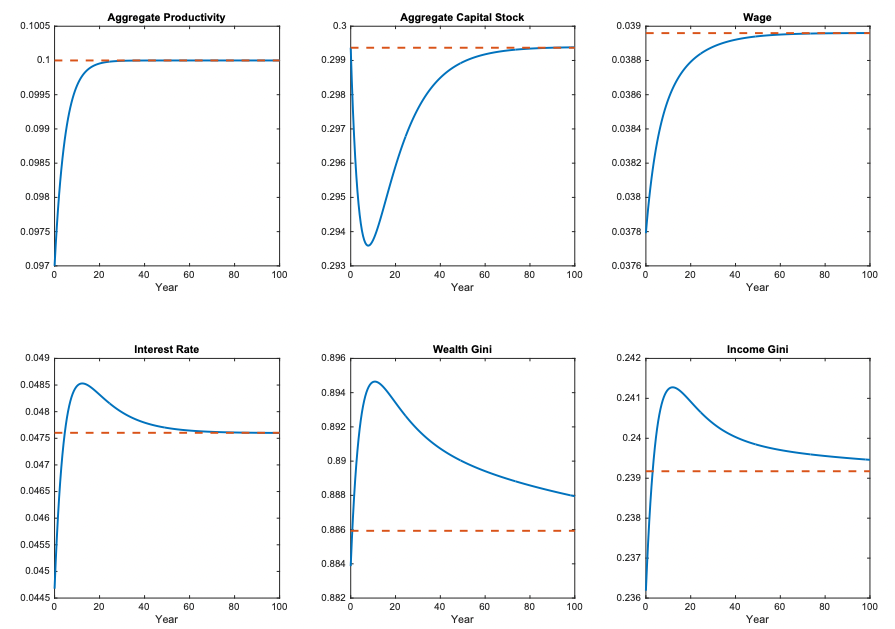
\includegraphics[width=.6\textwidth]{./figures/HACT_transition}
\end{frame}





%%%%%%%%%%%%%%%%%%%%%%%%%%  SLIDE   %%%%%%%%%%%%%%%%%%%%%%%%%%%%%%%%
\begin{transitionframe}
	{\color{white} \Huge \textbf{Generalizations and Applications} \vspace{2mm}}
\end{transitionframe}



\begin{frame}{A Model with a Continuum of Income Types}
\begin{itemize}
	\item Assume idiosyncratic income follows diffusion process
	$$dy_t = \mu(y_t)dt + \sigma(y_t)dW_t $$
	\item Reflecting barriers at $\ushort{y}$ and $\bar{y}$
	%\end{itemize}
	%\pause
	%\vspace{-3mm}
	%{\small \begin{align*}
			%\rho v(a,y) &=  \max_c \ u(c) + \partial_a v(a,y)(y + ra - c) + \mu(y)\partial_y v(a,y) + \frac{\sigma^2(y)}{2}\partial_{yy}v(a,y)\\
			%0 &= - \partial_a[s(a,y)g(a,y)] -\partial_y[\mu(y)g(a,y)] + \frac{1}{2}\partial_{yy}[\sigma^2(y)g(a,y)]\\
			%1 &= \int_{0}^\infty\int_{\ushort{a}}^\infty g(a,y)dady\\
			%B &= \int_0^\infty\int_{\ushort{a}}^\infty  a g(a,y)dady := S(r)
			%\end{align*}}
			%\begin{itemize}
			%\vspace{-3mm}
			%\item Borrowing constraint:  $\partial_a v(\ushort{a},y) \geq u'(y + r \ushort{a})$, all $y$
			%\smallskip
			%\item reflecting barriers (see e.g. Dixit ``Art of Smooth Pasting")
			%$$0 = \partial_y v(a,\ushort{y}) = \partial_y v(a,\bar{y})  $$ 
			%\pause 
			\bigskip
			\item Value function, distribution are now \tr{functions of 2 variables}:
			$$v(a,y) \quad \mbox{and} \quad g(a,y)$$
			\vspace{-1mm}
			\item $\Rightarrow$ HJB and KF equations are now \tr{P}DEs in $(a,y)$-space
		\end{itemize}
	\end{frame}


\begin{frame}
\vspace{2.5cm}
\begin{center}
	{\Large It doesn't matter whether you solve ODEs or PDEs}
	\\[2ex]
	{\Large $\Rightarrow$ everything generalizes}
\end{center}
\end{frame}




\begin{frame}{Saving Policy Function and Stationary Distribution}
\bigskip
\begin{figure}[ht]
	\centering
	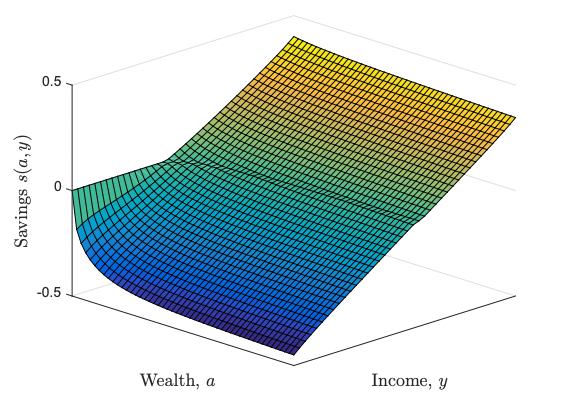
\includegraphics[width=.45\textwidth]{./figures/HACT_diffusion_savings} \qquad 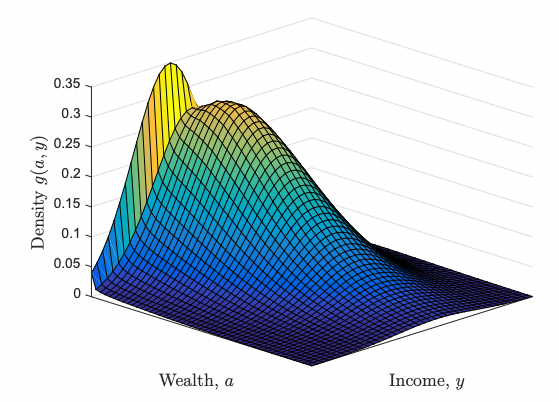
\includegraphics[width=.45\textwidth]{./figures/HACT_diffusion_distribution}
\end{figure}
\bi
\item Analytic characterization of MPCs: $c(a,y) \sim \sqrt{2 \nu(y)}\sqrt{a - \ushort{a}}$ with
\ei
{\small 
	\begin{align*}
		\nu(y) &= (\rho-r)\textrm{IES}(\ushort{c}(y))\ushort{c}(y) + \left(\mu(y) - \frac{\sigma^2(y)}{2}\mathcal{P}(\ushort{c}(y)) \right)\ushort{c}'(y) +  \frac{\sigma^2(y)}{2}\ushort{c}''(y)\\
		& \mbox{where} \ \mathcal{P}(c) :=-u'''(c)/u''(c) = \mbox{absolute prudence, and } \ushort{c}(y)=c(\ushort{a},y)
	\end{align*}
}
\end{frame}



\begin{frame}{Other Applications -- see Paper}
\bi
\item Non-convexities: indivisible housing, mortgages, poverty traps
\bigskip
\item Fat-tailed wealth distribution
\bigskip
\item Multiple assets with adjustment costs (Kaplan-Moll-Violante)
\bigskip
\item Stopping time problems
\ei
\end{frame}




%%%%%%%%%%%%%%%%%%%%%%%%%%  SLIDE   %%%%%%%%%%%%%%%%%%%%%%%%%%%%%%%%
%\begin{transitionframe}
%	{\color{white} \Huge \textbf{Open Questions} \vspace{2mm}}
%\end{transitionframe}





%%%%%%%%%%%%%%%%%%%%%%%%%%  SLIDE   %%%%%%%%%%%%%%%%%%%%%%%%%%%%%%%%
\begin{transitionframe}
	{\color{white} \Huge \textbf{Appendix} \vspace{2mm}}
\end{transitionframe}





\begin{frame}{Derivation of Poisson KF Equation  \hyperlink{equilibrium}{\beamergotobutton{Back}}}\label{KFEder}
\bi
\item Work with CDF (in wealth dimension)
$$G_j(a,t) := \Pr(\tilde{a}_t \leq a,\tilde{y}_t = y_i)$$
\item Income switches from $y_j$ to $y_{-j}$ with probability $\Delta \lambda_j$
\medskip
\item Over period of length $\Delta$, wealth evolves as $\tilde{a}_{t+\Delta} = \tilde{a}_t + \Delta s_j(\tilde{a}_t)$
\medskip
\item Similarly, answer to question ``where did $\tilde{a}_{t+\Delta}$ come from?" is
$$\tilde{a}_t = \tilde{a}_{t+\Delta} - \Delta s_j(\tilde{a}_{t+\Delta})$$
\item Momentarily ignoring income switches and assuming $s_j(a)<0$
\ei
{\small \begin{align*}
		\Pr(\tilde{a}_{t+\Delta} \leq a) = \underbrace{\Pr(\tilde{a}_{t} \leq a)}_{\textrm{already below $a$}} + \underbrace{\Pr(a \leq \tilde{a}_{t} \leq a - \Delta s_j(a))}_{\textrm{cross threshold $a$}} = \Pr(\tilde{a}_{t} \leq a - \Delta s_j(a))
\end{align*}}
\vspace{-2mm}
\bi
\item Fraction of people with wealth below $a$ evolves as
\begin{equation*}
	\begin{split}
		\Pr(\tilde{a}_{t+\Delta} \leq a,\tilde{y}_{t+\Delta}=y_j) = (1-\Delta \lambda_j)&\Pr(\tilde{a}_t \leq a - \Delta s_j(a),\tilde{y}_t = y_j)\\
		+ \Delta \lambda_j&\Pr(\tilde{a}_t \leq a - \Delta s_{-j}(a),\tilde{y}_t = y_{-j})
	\end{split}
\end{equation*}
\item Intuition: if have wealth $<a-\Delta s_j(a)$ at $t$, have wealth $<a$ at $t+\Delta$
\ei
\end{frame}


\begin{frame}{Derivation of Poisson KF Equation}
\begin{itemize}
	\item Subtracting $G_j(a,t)$ from both sides and dividing by $\Delta$
	{\small \begin{align*}
			\frac{G_j(a,t+\Delta) - G_j(a,t)}{\Delta} &= \frac{G_j(a - \Delta s_i(a),t) - G_j(a,t)}{\Delta}\\
			&- \lambda_jG_j(a - \Delta s_j(a),t) + \lambda_{-j}G_{-j}(a - \Delta s_{-j}(a),t)
	\end{align*}}
	\item Taking the limit as $\Delta \rightarrow 0$ 
	\tr{\begin{equation*}
			\partial_t G_j(a,t) = - s_j(a) \partial_a G_j(a,t) - \lambda_jG_j(a,t) + \lambda_{-j}G_{-j}(a,t)
	\end{equation*}}
	where we have used that 
	\begin{align*}
		\lim_{\Delta \rightarrow 0}\frac{G_j(a - \Delta s_j(a),t)-G_j(a,t)}{\Delta} &= \lim_{x \rightarrow 0}\frac{G_j(a - x,t)-G_j(a,t)}{x}s_j(a)\\
		&= -s_j(a) \partial_a G_j(a,t)
	\end{align*}
	\item Intuition: if $s_j(a)<0, \Pr(\tilde{a}_t \leq a,\tilde{y}_t=y_j)$ increases at rate $g_j(a,t)$ 
	\medskip
	\item Differentiate w.r.t. $a$ and use $g_j(a,t)=\partial_a G_j(a,t)$ $\Rightarrow$
	$$\partial_t g_j(a,t) = - \partial_a[s_j(a,t)g_j(a,t)] - \lambda_j g_j(a,t) + \lambda_{-j} g_{-j}(a,t)$$
\end{itemize}
\end{frame}




\begin{frame}{Accuracy of Finite Difference Method?}\label{sli:accuracy}
\bigskip
Two experiments:
\be
\medskip
\item special case: comparison with closed-form solution
\medskip
\item general case: comparison with numerical solution computed using very fine grid
\ee
\end{frame}




\begin{frame}{Accuracy of Finite Difference Method, Experiment 1}
\bi
\item Recall: get closed-form solution if
\bi
\smallskip
\item exponential utility $u'(c)=c^{-\theta c}$
\smallskip
\item no income risk and $r=0$ so that $\dot{a} = y - c$ (and $a \geq 0$)
\ei
\smallskip
$$\Rightarrow \qquad s(a) = -\sqrt{2\nu a}, \qquad c(a) = y + \sqrt{2\nu a}, \qquad \nu :=\frac{\rho}{\theta} $$
\item Accuracy with \tr{$I=1000$ grid points} ($\widehat{c}(a)$ = numerical solution)
\ei
\bigskip
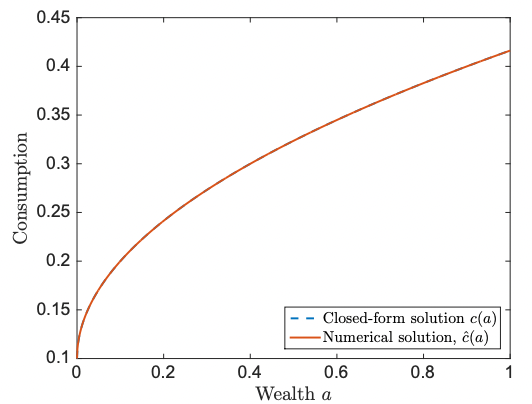
\includegraphics[width=.4\textwidth]{./figures/HACT_accuracy_consumption} \qquad 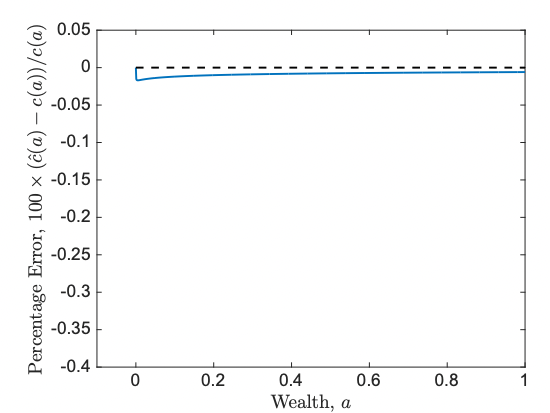
\includegraphics[width=.4\textwidth]{./figures/HACT_accuracy_error1000}
\end{frame}


\begin{frame}{Accuracy of Finite Difference Method, Experiment 1}
\bi
\item Recall: get closed-form solution if
\bi
\smallskip
\item exponential utility $u'(c)=c^{-\theta c}$
\smallskip
\item no income risk and $r=0$ so that $\dot{a} = y - c$ (and $a \geq 0$)
\ei
$$\Rightarrow \qquad s(a) = -\sqrt{2\nu a}, \qquad c(a) = y + \sqrt{2\nu a}, \qquad \nu :=\frac{\rho}{\theta} $$
\item Accuracy with \tr{$I=30$ grid points} ($\widehat{c}(a)$ = numerical solution)
\ei
\bigskip
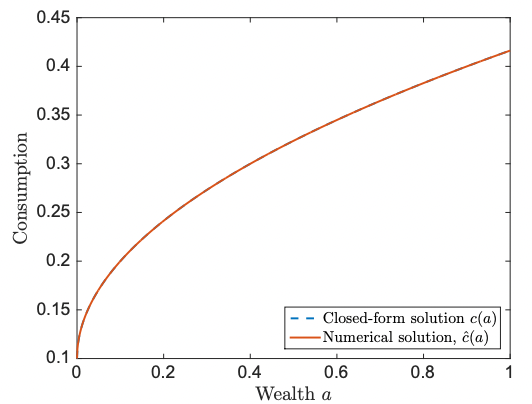
\includegraphics[width=.4\textwidth]{./figures/HACT_accuracy_consumption} \qquad 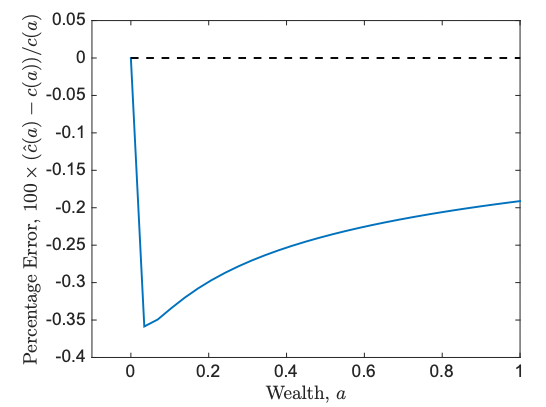
\includegraphics[width=.4\textwidth]{./figures/HACT_accuracy_error30}
\end{frame}


\begin{frame}{Accuracy of Finite Difference Method, Experiment 2}
\bi
\item Consider HJB equation with continuum of income types
{\small
	$$\rho v(a,y) =  \max_c \ u(c) + \partial_a v(a,y)(y + ra - c) + \mu(y)\partial_y v(a,y) + \tfrac{\sigma^2(y)}{2}\partial_{yy}v(a,y)$$}
\item Compute twice:
\be
\smallskip
\item with very fine grid: $I=3000$ wealth grid points
\smallskip
\item with coarse grid:  $I=300$ wealth grid points
\ee
\smallskip
then examine speed-accuracy tradeoff (accuracy = error in agg $C$)
\begin{table}
	\begin{tabular}{c|c|c}
		& Speed (in secs) & Aggregate $C$ \\
		\hline
		$I=3000$ & 0.916 & 1.1541 \\
		$I=300$ & 0.076 & 1.1606 \\
		\hline
		row 2/row 1 & 0.0876 &   1.005629\\
	\end{tabular}
\end{table}
\medskip
\item i.e. going from $I=3000$ to $I=300$ yields $>10 \times$ speed gain and $0.5\%$ reduction in accuracy (but note: even $I=3000$ very fast)
\medskip
\item Other comparisons? Feel free to play around with {\footnotesize \url{HJB_accuracy2.m}}
\ei
\end{frame}




\end{document}
